\chapter[Experiments on Estimating the Number of Sources]{One, Two, Three, Many: Experiments on Estimating the Number of Sources}
\label{cha:countanalysis}
\bigskip
\bigskip
\bigskip
\bigskip
%
The separation of mixtures into its original audio sources, as presented in the previous chapters, is a challenging task.
Furthermore, source separation is difficult to evaluate, and researchers compare to a known reference even though this does not reflect how humans separate mixtures.
It has long been a research topic to answer the question \emph{if} humans can separate, by fully extracting the desired source or if we can focus our attention on one source --- segregate them~\cite{bregman}.
Moreover, despite recent progress in auditory science~\cite{carlyon04, koelsch05, rabinowitz13}, research still is investigating how separation takes place in the auditory cortex or other parts of the human brain.
One thing, however, we can assess directly is if humans can reliably detect the number of sources in a mixture of several sources.
\par
In order to address this question, it helps to understand how humans infer counts and if our strategy is depending on the count.
When we look at vision, these are questions that have already been discussed over a hundred years ago in scientific research; an early study in the field of psychology of vision published by Jevons in 1871~\cite{jevons1871}.
He presented an experiment to quickly infer the number objects (beans) and came up with the hypothesis that humans can instantly estimate the number of objects without actually counting and therefore identifying them (``counting by detection'').
He mentioned in~\cite{jevons1871}:

\begin{quote}
``It is well known that the mind is unable through the eye to estimate any large number of objects without  counting them successively. A small number, for instance three or four, it can certainly comprehend and count by an instantaneous and apparently single act of mental attention.''
\end{quote}

This ``one-two-three-many'' hypothesis was a fundamental observation.
The fact that we can directly infer the numerosity of small numbers of objects, up to about four, is also known as \emph{subitizing}~\cite{kaufman49, burr10}.
I refer to this strategy as ``direct count estimation''.
Concerning our hearing, there are indications that the auditory system is capable of subitizing audio sources~\cite{hoopen79}.
And surprisingly, as shown in~\cite{kashino96, kawashima15}, humans share the same limitations of correctly estimate up to three simultaneously active speakers.
\par
In this chapter, I present two experiments contributing to this interesting field of research.
The first experiment (Section~\ref{sec:ismir}) addresses the question if the number of instruments in polyphonic music are subject to the same limitations.
In the second contribution (Section~\ref{sec:ismir}) the aim is to verify the findings of and earlier experiment in~\cite{kawashima15} and increase the number of stimuli to be used for comparison of machine learning based count estimations methods

\section{Instrument Count Estimation}%
\label{sec:ismir}

\marginpar{This chapter is based on the work that has been published in~\cite{stoeter13, schoeffler13} together with my collegue Michael Schoeffler. Based on my original idea, in both publications the two first authors contributed equally to the work.}

% From ISMIR
In psychoacoustics, a sequence of sounds grouped by the auditory system is known as an ``auditory stream'' which was coined by Bregman and Campbell in ~\cite{Bregman1971}.
In the past decades, a lot of experimental work related to ``auditory streams'' has been done~\cite{Bregman1990}.
A majority of these experiments were psychoacoustically motivated, e.~g. the stimuli used were mostly of simple type like sinusoids or noises.
Especially from a psychoacoustic point of view, music is a very complex sound signal which contains high-level information (e.~g. instrumentation and song lyrics).
When listening to music, this high-level information is also mentally processed by humans.
For developing auditory models, it could be helpful to know the maximum number of instruments humans are able to estimate when listening to music.
\par
% From ISMIR
In 1989, Huron conducted a musically motivated experiment related to stream segregation~\cite{Huron1989}. In his experiment he asked the participants for the number of voices in excerpts of organ music.
Huron defined a voice as a single ``line'' of sound, more or less continuous, that maintains a separate identity in a sound field or musical texture (an overview of voice definitions is given by Cambouropoulos in~\cite{Cambouropoulos2008}).
Huron came to the conclusion that the number of correctly identified voices is \emph{up to three}.
Later in 1996, Reuter~\cite{reuter96} has analyzed how combinations of different instruments are perceived which sets the focus on different instrumentation and not on denumerability.

% Based on Hurons work, we carried out an experiment where we asked musicians and non-musicians how many instruments they could hear in short pieces of music\cite{Stoter2013}. In contrast to Huron we addressed a more general case where voices are played by different instruments and not only by organ. In Huron's experiment the responses of the participants were time-varying for each stimulus. Another difference is that in Huron's experiment all six participants except one had a musical background whereas our experiment was also attended by a large group of non-musicians.

% dup? ICA!
% The perception of concurrent sound sources has been analyzed on different scales so far. Bregman's and McAdams' \cite{mcadams79} auditory stream theory can be seen as an analytical way of describing how sound events are perceived by the human auditory system. Unfortunately, it is difficult to model professionally produced music by auditory stream models because of its high complexity.
% However, none of them is motivated to model the perceived number of musical sources. Kashino et. al \cite{kashino1995} addresses the questions for concurrent speakers in a ``cocktail party'' like environment and found an upper limit of three voices humans can perceive. When the focus shifts to musical instruments as sources, research has to take concepts from musicology into account. Huron \cite{huron89} was the first who addressed this question in 1989 at a musically meaningful level. Huron asked for the number of voices within a piece of music, where by voices in musicology one can define it as a line of sound or note events (See~\cite{Cambouropoulos2008} for further definitions). Huron determined by experimental results that the number of correctly identified voices is up to three.
We wanted to take a first step by designing an experiment where we focus on polyphonic music of inhomogeneous timbre, where the question is: What is the number of instruments humans can estimate correctly?
Several results are addressed in this work include a possible upper limit of the number of perceived instruments, but also if one can see significant differences in performance of musicians compared to non-musicians.
Such results can be used in auditory modeling or as a pre-processing step for source separation algorithms.

\subsection{Experiment}
For the purpose of gaining more knowledge in understanding the human perception of multiple present instruments, an experiment was conducted. Huron selected voices from organ pieces only. We wanted to address the more general case where voices are played by different instruments.
As we set our focus on comparison between musicians and non-musician.
Our experiment was designed so that it respects the fact that the latter have only limited musical background.
\par
Although it might be interesting to have direct comparison with Huron's experiment, we agree that expanding the methods to an inhomogeneous timbre case is error prone. One reason is that there is reasonable doubt about the non-musicians understandings in terms of how a voice is defined. This is why we choose a trade-off with a more simplified experiment where we asked for the number of instruments instead of voices. Also whereas Huron \cite{huron89}  excluded subjects from his experiment because of their lower performance, we compared the results of both groups.

\subsection{Stimuli}

The selection of music items is crucial for our experiment setup. Usually music recordings have no ground truth metadata available to determine the actual number of instruments. Using annotated music like that from the RWC database~\cite{rwc} fulfills this requirement but lacks the possibility to remix, attenuate or suppress specific sources. This is important so that the experiment consists of equally grouped stimuli. Instead of the original RWC recordings, the annotated MIDI data itself was used as prototypes for the stimuli.

To make the counting task less ambiguous for the subjects, the instrumentation was chosen to be mostly constant during the music piece.
Therefore we calculated an ``instrumental stationarity'' metric.
The annotated MIDI files from \cite{rwc} were converted into piano roll representations for each instrument channel. This representation was then converted into a binary \emph{instrumentation activity matrix} $\mathbf{I}_{AM}\lbrack \mathbf{\underline{k}}_1 \vert \mathbf{\underline{k}}_2 \vert  ... \vert \mathbf{\underline{k}}_N \rbrack \in \{0,1\}$, where at each discrete time instant $i$ a vector $\mathbf{\underline{k}}_i$ indicates which instruments are active. The aim is then to select frames of length $N$ which are stationary by means of changes in instrumentation and activity. To get many items with a high instruments count, the maximum number of instruments within a frame was stored in a binary mask $\mathbf{\underline{k}}_{max}$ which was compared with all $\mathbf{\underline{k}}_{i=1...N}$ so that $(\vert\mathbf{\underline{k}}_{i} \oplus \mathbf{\underline{k}}_{max}\vert \leq 1) \lor (\mathbf{\underline{k}}_{i} = \underline{0})$. The resulting binary vector was smoothed with an averaging kernel of size $N$. By peak picking we got a list of possible candidates which contained a high stationarity in instrumentation.
Further the RWC files were filtered a priori to exclude items dominated by electronic instruments or singing voice. Table~\ref{tab:items} presents the selected 12 items representing pairs of one to six simultaneously present instruments. Each item is around seven seconds long. By cutting at note offsets we varied the lengths of the items to make it semantically more meaningful. Six items (notated as RM-C***) belong to the classical western music genre whereas the other items are of mixed genre.
\par
The MIDI excerpts were humanized and rendered by a sequencer software utilizing state-of-the-art commercial sampling products.
The process is similar to the dataset creation mentioned in Section~\ref{unison_dataset}.
The rendered files were processed with convolutive reverb to match the original recordings. 
In informal listening tests the quality of the renderings was evaluated. 
In addition, participants did not give negative feedback about the artificialness of the items during the laboratory experiment. Additionally a loudness normalization was applied according to EBU-R128\cite{EBU2011}. To avoid spatial cues the files were downmixed to mono at 16~bit/44.1~kHz.

\begin{table}[htb]
\center
\small
\begin{tabular}{cr@{.}lr@{.}lp{6cm}c}
\toprule[1.5pt]
RWC~ID & \multicolumn{2}{c}{Start~[s]} & \multicolumn{2}{c}{Dur.~[s]} & Instrumentation & \(k\)\\
\midrule
J021 & 46 & 5 & 6 & 6 & Piano, Contrabass~(pizz.) and Trumpet & 3\\
\hline
C001 & 0&0 & 9&0 & Bassoon & 1  \\
G047 & 35&3 & 8&3 & Violoncello & 1 \\
\hline
C016 & 0&9 & 7&6 & Viola and Violoncello & 2\\
G068 & 132&4 & 6&6 & Violin and Flute &  2\\
\hline
C018 & 240&4 & 5&4 & French~Horn, Piano and Violin & 3\\
G046 & 0&3 & 7&9 & Contrabass, Piano and Violoncello & 3\\
\hline
C013 & 5&6 & 6&0 & Flute, Viola, Violin and Violoncello & 4\\
G036 & 0&0 & 6&5 &  Acoustic~Guitar, Electric~Bass, Piano  and Violin & 4\\
\hline
C012 & 112&0 & 6&0 & Contrabass, Flute, Viola, Violin and  Violoncello & 5\\
G037 & 67&1 & 7&0 & Acoustic~Guitar, Contrabass~(pizz.), Flute, Piano and Tenor~Sax & 5\\
\hline
C001 & 147&8 & 6&0 & Bassoon, Clarinet, Contrabass, French~Horn, Oboe and Violin & 6\\
G028 & 17&5 & 6&5 & Electric~Bass, Electric~Guitar, Flute, Piano, Trombone and Trumpet & 6\\
\bottomrule[1.5pt]
\end{tabular}
\caption{Selected items from the RWC Music Database \cite{rwc}. Item \emph{J021**} is used as training item.}
\label{tab:items}
\end{table}

\subsection{Methods and Participants}
The experiment was attended by 62 participants, where half of them regularly play a musical instrument. They were asked to count how many different instruments they can hear. 12 items from the test set (Table~\ref{tab:items}) were played back in random order. The experiment was presented by a user interface depicted in Figure~\ref{fig:experiment_ui}. Except for the training item, every subject could play back each stimulus up to three times. Additionally they were asked to estimate how certain they were in their decision (ranged from \emph{uncertain} to \emph{very certain}).
\begin{figure}[h]
	\centering
		\fbox{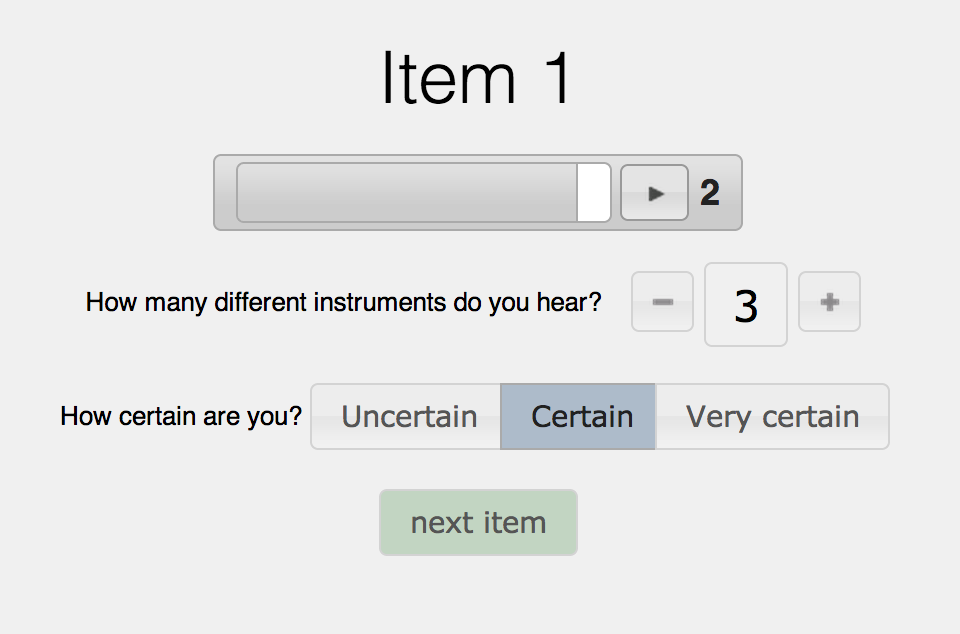
\includegraphics[width=3in]{Chapters/07_Analysis_Experiment/figures/user_interface.png}}
	\caption{Experiment User Interface}
	\label{fig:experiment_ui}
\end{figure}
Instead of a slider UI-element, the interface only features plus and minus buttons so that the subjects were not biased about the maximum number of instruments. Item \emph{J021**} had been selected as training item and was presented to the subjects during the introduction phase to make them familiar with the user interface. This trial also unveiled the number and name of the instruments within that piece. After they had read the introduction page, the subjects were asked to adjust the volume during the training example to their preference and leave the volume at that level for the duration of the experiment. The stimuli were presented on \textsc{Beyerdynamics DT770} headphones connected to a \textsc{RME Babyface}. The complete test took about 20 minutes on average for every participant.

\subsection{Results: A gap of one instrument}

\begin{figure}[h]
\centering
\begin{minipage}{0.8\textwidth}
\begin{tabular}{c}
	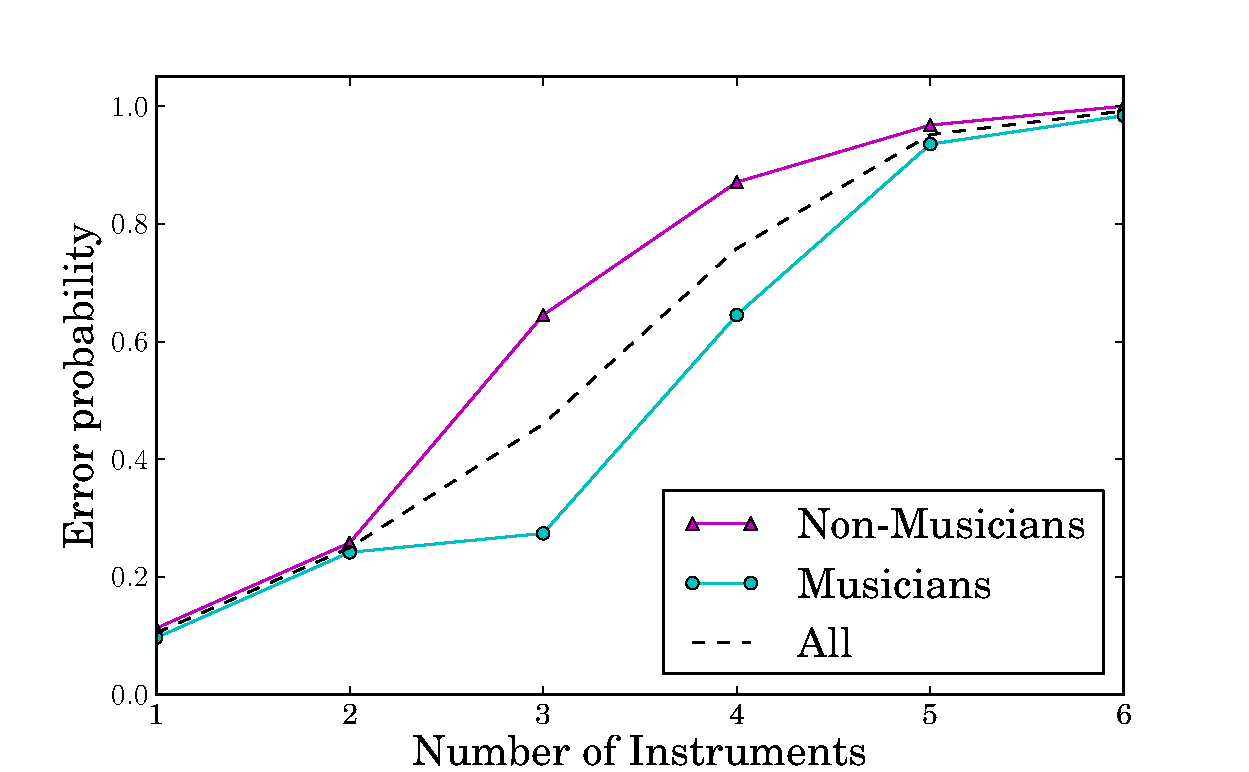
\includegraphics[width=\textwidth]{Chapters/07_Analysis_Experiment/images/error_means.pdf}
\end{tabular}
\end{minipage}
\\
\begin{minipage}{0.8\textwidth}
\begin{tabular}{c}
	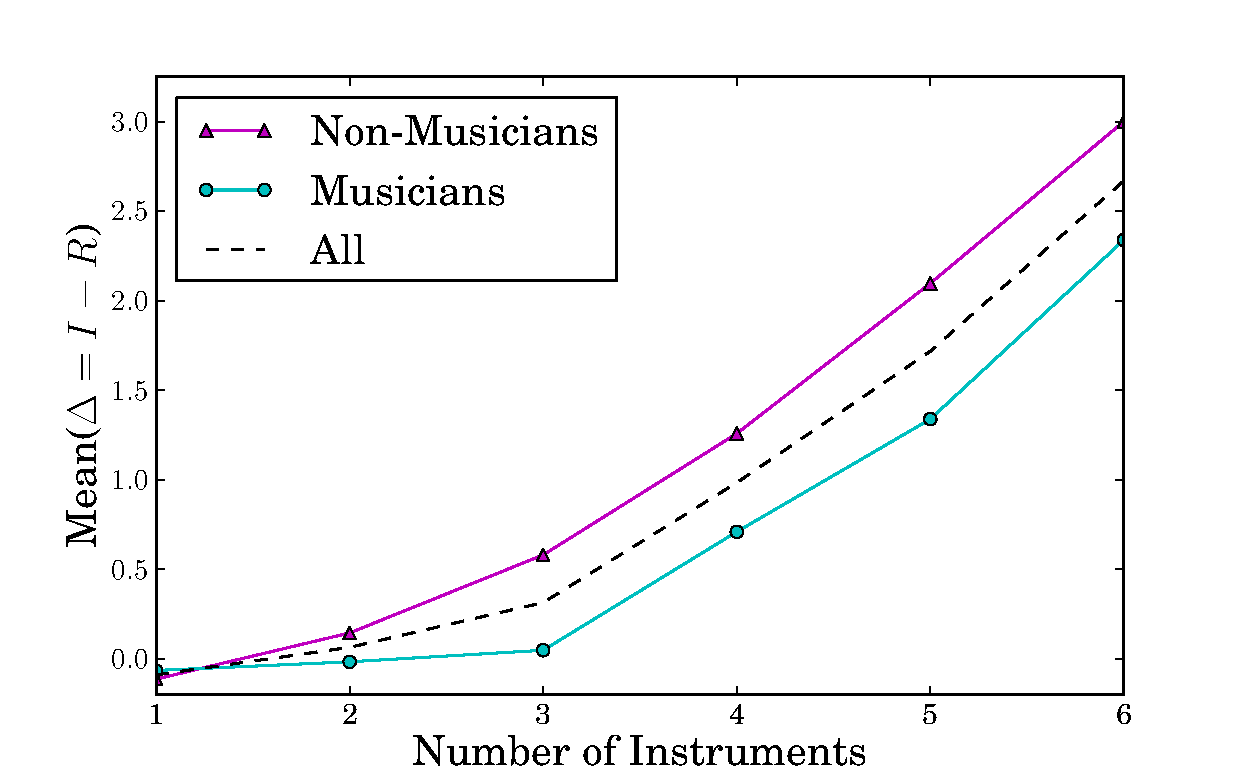
\includegraphics[width=\textwidth]{Chapters/07_Analysis_Experiment/images/error_diff.pdf}
\end{tabular}
\end{minipage}
\caption{Error probability (top) and Mean of $\Delta = I-R$ (right) categorized by the number of instruments.}
\label{fig:meanerror}
\end{figure}

The independent variable $I(i)$ is the number of instruments of one music item $i$ where in this case $I(i) \in \{1,2,...,6\}$. $R(i,s)$ is defined as the number of instruments that are perceived and counted by subject $s$ for music item $i$. The dependent variable is the derived from the main subject response as $\Delta(i,s) = I(i) - R(i,s)$ transformed into a binary scale:
\begin{align}%
\label{eq:response}
	E(i,s)&=\begin{cases}
		0 & \text{if $|\Delta| = 0 $ } \\
		1 & \text{if $|\Delta| > 0 $ .}\\
	\end{cases}
\end{align}
\par
The primary statistical null hypothesis ($H_1$) is stated in that the means of $\Delta$ and $E$\footnote{The fact that $E$ is dichotomous will lead to a mean value that equals to a probability of a binary distribution.}, grouped by the number of instruments, do not differ significantly. As we also want to test the between-groups performance of musicians versus non-musicians, we introduce another dependent variable $M(s) \in \{0,1\}$ of binary scale. This is stated in a secondary null hypothesis ($H_2$) where the means of $\Delta$ and $E$ are not significantly different between musicians and non-musicians.
No subjects were screened from the results, although there are two cases where no valid response had been made. Results are grouped by items of $I$ instruments.
\par
In general participants tended to perform worse for items with more than two instruments. The probability of correctly counting one instrument was 90.0\% whereas only one person out of 62 gave a correct response for an item with six instruments. In some cases the number of instruments does not correspond to the number of voices for every item. Items where an instrument plays more than one voice and voices which are played by more than one instrument. However most of the chosen instruments are monophonic so in our case this occurred only for items where piano or guitar is present. Also we made sure that the number of total voices did not exceed the maximum number of instruments in that item. Voices being played by more than one instrument are called unison, which is present in G068, that showed surprisingly good results.

\subsubsection*{Underestimation}

We confirmed the results in~\cite{huron89} that the most common error is the underestimation of one instrument, although this accounts only for 43 \% of the responses in our experiment. Only in one case $\Delta$ is negative (overestimation) which is item C016, a ``Clarinet Quintet in A major by Wolfgang Amadeus Mozart (K.581. 1st mvmt)'' where we have excluded the solo clarinet part and two strings. Still, the remaining sound seems to be so similar to that of a quartet that musicians tended to hear ``phantom'' instruments.

\subsubsection*{Main Effects}

To test the null hypotheses ($H_1$ and $H_2$), statistical tools are required.
The first tests focus on $\Delta$ which is an interval scaled variable. To show differences between means of two or more groups, usually One-Way-ANOVA tests are applied. ANOVA tests expect independent normally distributed variables and homogeneity of the variances in each group. However both the Kolmogorov--Smirnov test of normal distribution and Levene's test to determine the homogeneity of group variances fail. In such cases variables scaled like $\Delta$ could be transformed so that the boundaries are straightened out. A typically used $arcsin(\sqrt{\Delta})$ transformation was applied to $\Delta$ resulting in slightly higher $p$ values but still not statistically significant. Although ANOVA is known to be robust enough to run the tests against non-normal distributed cases and unequal variances, the significance levels of the results are doubtful. Therefore we choose to run a non-parametric test. The Kruskal--Wallis test can be applied even if the data is not normally distributed. However it has to be run on a slightly modified hypothesis which compares the medians of groups instead of the means. The Kruskal--Wallis test allows to reject both modified hypotheses (asymptotic $p = 0.000$, $\chi^2 = 499636$, $df=5$).
% As mentioned by \cite{fagerland2009} it may be crucial for the Kruskal--Wallis test to be run on groups with differently shaped distributions.
%  This may not be assured in the case of $\Delta$ as the skewness highly increases for $I \geq 3$. Although the significance of the test has to be treated with caution, the median is a good indicator of a possible upper limit. The overall medians for all groups are plotted in Figure~\ref{fig:median} where one can see that three instruments are a possible upper bound.
\par
Concerning $E$ which is a categorical variable, linear models such as ANOVA cannot be used.
As described in~\cite{jaeger08}, instead, a binary regression model that turns the mean of $E$ into a an binomial distributed probability, can be used.
Similar to ANOVA, the output variable will be modeled by a \emph{binary logit regression} that models the output using \emph{log linear} values.
\par
By including the main factors $I$ and $M$ we set up a \emph{Generalized Linear Model} (GLM)
\begin{equation}
	logit(E) =  \text{Intercept} + x_1 \text{I} + x_2 \text{M} .
	\label{eq:logit_main}
\end{equation}
A test of the main effects is statistically significant ($\chi^2$ = $437418$, $p < 0.000$, $df = 6$) so that both null hypotheses ($H_1$ and $H_2$) can be rejected. The significance of both effects as well as parameter estimates and Wald values of the calculated model are shown is shown in~\cite{stoeter13}.
The results indicate that there is a significant difference in the error probability for groups of instrumentation counts but also for musicians versus non-musicians. A pairwise comparison test based on the mean differences reveals where these differences are located. Regarding the error probability of different instrument counts, the pairwise comparison test reveals that nearly all groups show significant mean differences between each other, which was the expected result. However, by calculation using the logit GLM model shown in equation~\ref{eq:logit_main} we found that there are two groups of items of five and six instruments (mean difference $0.04$, std. error = $0.019$, $df = 1$, $p = 0.055$) that did not show any significant difference. For both groups the error probability is close to 100\%.
\par
To investigate the difference in performance between musicians and non-musicians a pairwise comparison between those two groups was run. Overall musicians perform about 20\% better throughout the test (mean difference = $0.18$, std. error = $ 0.0044$, $df = 1$, $p=0.000$). We do not know what caused these differences as the level of professionalism had not been surveyed. Also 37 \% of the musicians additionally had experience in audio engineering due to their profession.
\par
Further, to look at possible interaction effects between the number of instruments and the groups of musicians and non-musicians we adapted our logit equation to
\begin{equation}
	logit(E) =  \text{Intercept} + x_1 \text{I} + x_2 \text{M} + x_3 \text{M}\times\text{I} .
	\label{eq:logit_interactions}
\end{equation}
We then reran the GLM analysis selecting only items of three and four instruments. This avoids quasi-complete separation in the logit regression model which is caused by low variances in the error probability for items of $I \in \{1,2,5,6\}$.
The model effects of the subset can be found in~\cite{stoeter13}.
% \begin{table}
% \center
% \scriptsize
% \begin{minipage}[b]{0.45\textwidth}\centering
% 	\begin{tabular}{rccc}
% 	\toprule[1.5pt]
% 	Source    & Wald $\chi^2$ & df & p \\
% 	\midrule
% 	Intercept & 22.643 & 1 & 0.000 \\
% 	I & 185.359	& 5 & 0.000 \\
% 	M & 17.977 & 1 & 0.000 \\
% 	& & & \\
% 	\bottomrule[1.5pt]
% 	\end{tabular}
% 	\caption{Tests of Model Effects of dependent variable $E$ }
%     \label{tab:glm_logit}
% \end{minipage}
% \hfill
% \begin{minipage}[b]{0.45\textwidth}
% 	\begin{tabular}{rccc}
% 	\toprule[1.5pt]
% 	Source    & Wald $\chi^2$ & df & p \\
% 	\midrule
% 	Intercept & 12.434 & 1 & 0.000 \\
% 	I & 22.742	& 1 & 0.000 \\
% 	M & 22.742 & 1 & 0.000 \\
% 	M$\times$I	& 0.184 & 1 & 0.668 \\
% 	\bottomrule[1.5pt]
% 	\end{tabular}
% 	\caption{Tests of Model Effects of dependent variable $E$ for a subset of items with $I \in \{3,4\}$}
%     \label{tab:glm_logit_34}
% \end{minipage}
% \end{table}

\begin{figure}[h]
	\centering
	\scriptsize
	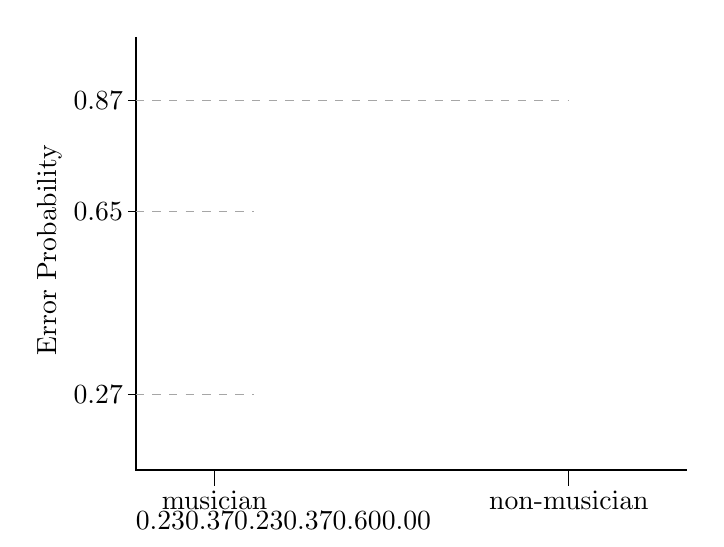
\begin{tikzpicture}[node distance=2cm]
		\draw [-,thick] (0,5*1.25) node (yaxis) [left] {$ $}
	        |- (7,0.75) node (xaxis) {$ $};

		\draw (-1.1, 5) node[left,rotate=90] {Error~Probability};

		\draw (1,-0.2+0.75) -- (1,0+0.75) node[below=4pt] {musician};
		\draw (5.5,-0.2+0.75) -- (5.5,0+0.75) node[below=4pt] {non-musician};

	%	\draw (-0.1, 0) -- (0.1, 0) node[left=4pt] {$0\%$};
		\draw (-0.1, 1.3710*1.25) -- (0.1, 1.3710*1.25) node[left=4pt] {$0.27$};
		\draw (-0.1, 3.2258*1.25) -- (0.1, 3.2258*1.25) node[left=4pt] {$0.65$};
		\draw (-0.1, 4.3548*1.25) -- (0.1, 4.3548*1.25) node[left=4pt] {$0.87$};
	%	\draw (-0.1, 5*1.25) -- (0.1, 5*1.25) node[left=4pt] {$100\%$};

		\draw[dashed,style={color=black!35}] (0, 1.3710*1.25) -- (1.5, 1.3710*1.25) node[left=4pt] {};
		\draw[dashed,style={color=black!35}] (0, 3.2258*1.25) -- (1.5, 3.2258*1.25) node[left=4pt] {};
		\draw[dashed,style={color=black!35}] (0, 4.3548*1.25) -- (5.5, 4.3548*1.25) node[left=4pt] {};

		\GraphInit[vstyle=Normal]
		\tikzset{EdgeStyle/.style={}}
		\tikzset{colorstyle/.style={
			shape= circle,
			line width = 1pt,
			draw = black,
			fill = #1!30}
		}

		\Vertex[L=3,x=1,y=1.3710*1.25,style={colorstyle=red,line width = 4pt}] {3M}
		\Vertex[L=4,x=1,y=3.2258*1.25,style={colorstyle=blue,line width = 2pt}] {4M}
		\Vertex[L=3,x=5.5,y= 3.2258*1.25,style={line width = 4pt}] {3N}
		\Vertex[L=4,x=5.5,y=4.3548*1.25,style={colorstyle=green, draw = black!0,line width = 0}] {4N}

		\Edge[label=$0.23$,style={color=black!50}](3N)(4N)
		\Edge[label=$0.37$,style={color=black!50}](3N)(3M)

		\Edge[label=$0.23$,style={color=black!50}](4N)(4M)
		\Edge[label=$0.37$,style={color=black!50}](4M)(3M)
		\Edge[label=$0.60$,style={color=black!50}](3M)(4N)
		\Edge[label=$0.00$,style={color=red, line width = 2pt}](3N)(4M)

		\end{tikzpicture}
		\caption{Pairwise comparison between interaction of Musician/Non-Musician and the number of instruments (labeled in nodes). The costs between nodes indicates the mean differences between groups. The red/bold line indicates that is there is no significant difference at the $p=0.005$ level}
		\label{fig:graph}
\end{figure}
The results indicate that interaction of Musician$\times$Instruments is not significant on a $p=0.05$ level in general and a pairwise comparison test reveals two groups of equal probability. The pairwise comparisons are depicted in Figure~\ref{fig:graph}. The red vertex indicates there is no significant difference in the error probability for the group of musicians in items with four instruments compared to non-musicians in items of three instruments. Therefore a gap in the error probability of one instrument between those two groups becomes apparent.

\subsection{Large Internet Experiment}
It has been becoming more and more popular to use the Internet for experiments in music or auditory perception. One of the first auditory experiments were conducted by Welch and Krantz\cite{Welch1996} in 1996. A web experiment related to MIREX tasks using \emph{Amazon Mechanical Turk} has been conducted by Lee \cite{lee2010}. An experiment with a large attendance was done by Salganik~\textit{et~al.}\cite{Salganik2006} in 2006. They had over 14.000 participants and examined the social influence on participants in an artificial music market. An overview of recent Internet experiments is given by Reips\cite{Reips2012}.
\par
For many types of music perception experiments such as estimating the number of instruments, it is essential that the selected participants represent a large population. As recent research in cross-cultural music perception and cognition reveals: The perception of music is dependent on the origin of people\cite{stevens2012}. Besides the cultural background, other aspects like their profession might have an influence when estimating the number of instruments being played back, e.~g. musicians might recognize instruments much more easily since they are in touch with instruments in their everyday life. One of the advantages of Internet experiments (also called web-based experiments or web experiments) is that it is easier to gather participants with different backgrounds and from different regions than in laboratory experiments. For a summary of benefits and disadvantages of Internet experiments see \cite{Reips2002}. In music perception a major argument against Internet experiments is that there is no control about the environment. With the spreading of mobile devices with Internet connections this argument becomes more apparent, since the environment of the participants can range from a quiet place at home to a noisy place outside.
\par
By comparing the results of the Internet experiment to the results of the same experiment but previously conducted in a controlled environment as presented in the previous section, we contribute to answering the research question, whether the Internet can be used for experiments in music perception.
Furthermore, subpopulations like headphones-users and loudspeaker-users are examined whether they lead to more reliable responses.
\par
Participation in the experiment was done by visiting the experiment's website\footnote{{\scriptsize\url{http://www.audiolabs-erlangen.com/experiments/wice/}}}. The experiment was promoted in mailing lists, forums, social networks and by personal invitations. Most of the forums and mailing lists were audio-related. No material incentive was given to participants. For motivating the participants a high score was added to the experiment.
\par
In total 1310 website visitors attended the experiment.
We identified 115 of them as participants who did the experiment more than once by using a browser fingerprinting method (for more details in browser fingerprinting, see~\cite{Eckersley2010}).
In this case, only the first trial is used in the results analysis.
Our browser fingerprinting method created a hash value by using the visitor's browser settings, e.~g. screen resolution and installed plugins. In addition, we excluded 27 participants since they gave at least one non-serious response. We defined responses with zero instruments (25~participants) and responses with more than 12 instruments (two participants) as invalid. After the screening we had 1168 valid participants.
\par
The participants were asked by a questionnaire whether they have a professional background in audio, play at least one instrument (including singing) and are familiar with listening tests. Detailed information about the participants are described in~\cite{schoeffler13}.
% \begin{table}[htb]
% \center
% \scriptsize
% \renewcommand{\arraystretch}{1.2}
% %\begin{tabular}{cr@{.}lr@{.}lr@{.}l}
% \begin{tabular*}{0.45\textwidth}{c r@{ }l r@{ }l r@{ }l r@{ }l r@{ }l}
% \toprule[1.5pt]
% Total & \multicolumn{2}{c}{Age group} & \multicolumn{2}{c}{Musician} & \multicolumn{2}{c}{Professional} & \multicolumn{2}{c}{Headphones} \\
% \midrule
% 1168 &  0  & [0-12]  & -   &  	   & -   &       & -   &       \\
%  	 \cline{2-9} \rule{0pt}{10pt}
%      & 110 & [13-19] & 74  & [yes] & 12  & [yes] & 5   & [yes] \\
%      &     &         &	   &       &     &       & 7   & [no]  \\
%      &     &   		 &     &       & 62  & [no]  & 30  & [yes] \\
%      &     &         &	   &       &     &       & 32  & [no]  \\
%      &     &   		 & 36  & [no]  & 0   & [yes] & -   &       \\
%      &     &         &	   &       &     &       & -   &       \\
%      &     &   		 &     &       & 36  & [no]  & 17  & [yes] \\
%      &     &         &	   &       &     &       & 19  & [no]  \\
%      \cline{2-9} \rule{0pt}{10pt}
%      & 889 & [20-39] & 463 & [yes] & 128 & [yes] & 81   & [yes] \\
%      &     &         &	   &       &     &       & 47   & [no]  \\
%      &     &   		 &     &       & 335 & [no]  & 154  & [yes] \\
%      &     &         &	   &       &     &       & 181  & [no]  \\
%      &     &   		 & 426 & [no]  & 46  & [yes] & 31   & [yes] \\
%      &     &         &	   &       &     &       & 15   & [no]  \\
%      &     &   		 &     &       & 380 & [no]  & 164  & [yes] \\
%      &     &         &	   &       &     &       & 216  & [no]  \\
%      \cline{2-9} \rule{0pt}{10pt}
%      & 143 & [40-59] & 98 & [yes] & 32  & [yes] & 22   & [yes] \\
%      &     &         &	  &       &     &       & 10   & [no]  \\
%      &     &   		 &    &       & 66  & [no]  & 31   & [yes] \\
%      &     &         &	  &       &     &       & 35   & [no]  \\
%      &     &   		 & 45 & [no]  & 8   & [yes] & 5    & [yes] \\
%      &     &         &	  &       &     &       & 3    & [no]  \\
%      &     &   		 &    &       & 37  & [no]  & 17   & [yes] \\
%      &     &         &	  &       &     &       & 20   & [no]  \\
%      \cline{2-9} \rule{0pt}{10pt}
%      & 26  & [60+]   & 13 & [yes] & 6   & [yes] & 3    & [yes] \\
%      &     &         &	  &       &     &       & 3    & [no]  \\
%      &     &   		 &    &       & 7   & [no]  & 4    & [yes] \\
%      &     &         &	  &       &     &       & 3    & [no]  \\
%      &     &   		 & 13 & [no]  & 2   & [yes] & 2    & [yes] \\
%      &     &         &	  &       &     &       & 0    & [no]  \\
%      &     &   		 &    &       & 11  & [no]  & 5    & [yes] \\
%      &     &         &	  &       &     &       & 6    & [no]  \\
% \bottomrule[1.5pt]
% \end{tabular*}
% \caption{Information about the participants.}
% \renewcommand{\arraystretch}{1}
% \label{table:info_participants}
% \end{table}
\par
The main functionality of the experiment's website was written in HTML5 and JavaScript. The stimuli were presented as uncompressed wav, where possible\footnote{Since some browsers (e.~g. Internet Explorer) did not support WAV, MP3 (encoded with \SI{256}{kbits/s} CBR with Fraunhofer Encoder) was used as alternative file format}.
\par
The experiment started on February the 15th, 2013 and lasted until March the 15th, 2013.
At first, participants filled out a short questionnaire. They were asked which audio setup they are using, whether they regularly play any musical instruments or do singing, have a background in professional audio, are familiar with listening tests and which age group they belong to.
\par
After filling out the questionnaire, the participants did a short training. The purpose of the training was to familiarize the participants with the user interface and to give them the option to adjust the volume. The training had one stimulus with three instruments being played. The instruments were piano, bass and trumpet. The participants were told on the training page how many and which instruments are played back. During the training it was possible to listen to the stimulus unlimited times.

\subsection{Results}\label{sec:results}

The independent variables are the number of instruments being played back ($\textit{Num}_{\mathrm{Inst}}$), whether a participant is musical ($\textit{Musical}$), professional in audio ($\textit{Professional}$) and which setup was used ($\textit{Setup}$). A participant is defined as musical ($\textit{Musical} = true$) when he or she is regularly playing an instrument (including singing). The same applies to being professional ($\textit{Professional} = true$) which is set when the participant responded that he or she is a professional in audio. The responses for the setup used can either be headphones ($\textit{Setup} = \textrm{`}headphones\textrm{'}$) or loudspeaker ($\textit{Setup} = \textrm{`}loudspeaker\textrm{'}$). The dependent variable is the participant's estimation of the number of instruments being played back ($\textit{Resp}$). A correct estimation is the inverse of Equation~\ref{eq:response}.
% \begin{equation}
% \label{equation:response_correct}
% \textit{Resp}_{\mathrm{Correct}} =
% \begin{cases}
% 0 & \text{if } \text{\textit{Num}}_{\mathrm{Inst}} \neq \text{\textit{Resp}}
% \\
% 1 & \text{if } \text{\textit{Num}}_{\mathrm{Inst}} = \text{\textit{Resp}}
% \end{cases}
% \mathrm{.}
% \end{equation}

% Table~\ref{table:responses} shows the responses of the participants for all stimuli.
% \tabcolsep=5.5pt
% \begin{table}[t]
% \tiny
% \begin{tabular}{p{1cm}ccccccc}
% \toprule[1.5pt]
%  & \multicolumn{ 7}{c}{$\textit{Num}_{\mathrm{Inst}}$} \\
%   \cmidrule(l){2-8}
%  $\textit{Resp}$ & $I=1$ & $I=2$ & $I=3$ & $ I=4$ & $I=5$ & $I=6$ & n \\

%  \midrule
%  $R=1$ & \cellcolor[gray]{0.9} 2025 & 373 & 5 & 18 & 13 & 12 & 2446 \\
%  \midrule
%  $R=2$ & 298 & \cellcolor[gray]{0.9} 1642 & 810 & 736 & 451 & 382 & 4319 \\
%  \midrule
%  $R=3$ & 12 & 277 & \cellcolor[gray]{0.9} 1343 & 1145 & 1093 & 1069 & 4939 \\
%  \midrule
%  $R=4$ & 1 & 43 & 158 & \cellcolor[gray]{0.9} 386 & 645 & 680 & 1913 \\
%  \midrule
%  $R=5$ & 0 & 1 & 18 & 48 & \cellcolor[gray]{0.9} 120 & 155 & 342 \\
%  \midrule
%  $R=6$ & 0 & 0 & 1 & 3 & 12 & \cellcolor[gray]{0.9} 30 & 46 \\
%  \midrule
%  $R>6$ & 0 & 0 & 1 & 0 & 2 & 8 & 11 \\

%  \midrule
%  & \multicolumn{7}{c}{14016 responses (1168 participants $\cdot$ 12 items)} \\
% \midrule[1pt]

% Probability of $\textit{Resp}_{\mathrm{Correct}}$ & 0.87 & 0.70 & 0.57 & 0.17 & 0.05 & 0.01 &  \\

%  \bottomrule[1.5pt]
% \end{tabular}
% \caption{Responses from the participants. The cells with a gray background represent correct estimations.}
% \label{table:responses}
% \end{table}
% \tabcolsep=6pt

For testing hypotheses, a logistic regression model with the response variable $\textit{Resp}_{\mathrm{Correct}}$ and the predictor variables $\textit{Num}_{\mathrm{Inst}}$, $\textit{Musical}$, $\textit{Professional}$ and $\textit{Setup}$ was calculated.
The estimated coefficients, p-values and average marginal effects can be found in~\cite{schoeffler13}.
% \tabcolsep=5.5pt
% \begin{table}[t]
% \center
% \scriptsize
% \begin{tabular}{p{1.5cm}ccccp{0.8cm}}
% \toprule[1.5pt]
% Coefficient & Estimate & Std. Error & z-value & p-value & Average Marginal Effects \\
% \midrule
% (Intercept) & 1.5015 & 0.06836 & 21.963 & \textless~2e-16 & 0.1886 \\
% $\textit{Num}_{\mathrm{Inst}} = 2$ & -1.0293 & 0.07651 & -13.453  & \textless~2e-16 & -0.1293\\
% $\textit{Num}_{\mathrm{Inst}} = 3$ & -1.6021 & 0.07463 & -21.466  & \textless~2e-16 & -0.2012\\
% $\textit{Num}_{\mathrm{Inst}} = 4$ & -3.5674 & 0.08380 & -42.572  & \textless~2e-16 & -0.4481\\
% $\textit{Num}_{\mathrm{Inst}} = 5$ & -4.8759 & 0.11290 & -43.188  & \textless~2e-16 & -0.6125\\
% $\textit{Num}_{\mathrm{Inst}} = 6$ & -6.3061 & 0.19428 & -32.459  & \textless~2e-16 & -0.7922\\
% $\textit{Musical} = true$ & 0.5266 & 0.04932 & 10.676  & \textless~2e-16 & 0.0661\\
% $\textit{Professional} = true$ & 0.3306 & 0.06234 & 5.303  & 1.14e-07 & 0.0415\\
% $\textit{Setup} = \textrm{`}headphones\textrm{'}$ & 0.1071 & 0.04823 & 2.220  & 0.0264 & 0.0135\\
% \midrule
% \multicolumn{6}{l}{(Dispersion parameter for binomial family taken to be 1)}\\
% \multicolumn{6}{l}{Null deviance: 18816  on 14015  degrees of freedom}\\
% \multicolumn{6}{l}{Residual deviance: 11036  on 14007  degrees of freedom}\\
% \multicolumn{6}{l}{AIC: 11054}\\
% \multicolumn{6}{l}{Number of Fisher Scoring iterations: 7}\\
% \multicolumn{6}{l}{McFadden's Pseudo R-squared: 0.413}\\
% \bottomrule[1.5pt]
% \end{tabular}
% \tabcolsep=6pt
% \caption{Logit regression model for response variable $\textit{Resp}_{\mathrm{Correct}}$ calculated from the data obtained by the Internet experiment.}
% \label{table:data_web_lm}
% \end{table}
% Average marginal effects in the regression model describe the increase in proportion of correct responses of estimating the number of instruments when the predictor variable is increased by one level.
% \par
% As expected, participants who play an instrument or do singing ($\textit{Musical} = true$) performed slightly better than non-musicians. According to the average marginal effect their chance of estimating the number of instruments correctly is $6.61\%$ more likely for all stimuli. A similar increase for estimating the number correctly ($4.15\%$) can be seen for participants being a professional in audio ($\textit{Professional} = true$).
The average marginal effects of $\textit{Num}_{\mathrm{Inst}}$ indicates up to which point humans are able to correctly estimate the number of instruments being played back. The average marginal effect of $\textit{Num}_{\mathrm{Inst}} = 2$ shows that it is $12.93\%$ less likely to estimate correctly when listening to two instruments instead of one instrument. Furthermore, in case of three instruments being played back the probability of estimating the wrong number increases to $20.12\%$. The highly negative average marginal effect of $-0.4481$ for $\textit{Num}_{\mathrm{Inst}} = 4$ indicates that it is very unlikely for humans to estimate the number of instruments correctly compared to estimating the number of one to three instruments. This, we confirmed the results of our laboratory experiment.
\cite
For a detailed analysis of the differences between the Internet experiment and the laboratory experiment in a controlled environment, a second logit regression model was calculated. This logit regression model includes the data of the previous experiment which has responses of 62 participants and also added an additional predictor variable $\textit{Environment}$.
The model fit output can be found in~\cite{schoeffler13}.
% escribed in Table~\ref{table:data_both_lm}).
% \begin{table}[t]
% \center
% \scriptsize
% \begin{tabular}{p{1.5cm}ccccp{0.8cm}}
% \toprule[1.5pt]
% Coefficient & Estimate & Std. Error & z-value & p-value & Average Marginal Effects \\
% \midrule
% (Intercept) & 2.0226 & 0.11718 & 17.260 & \textless~2e-16 & 0.2590\\
% $\textit{Num}_{\mathrm{Inst}} = 2$ & -1.0135 & 0.07424 & -13.652  & \textless~2e-16 & -0.1298\\
% $\textit{Num}_{\mathrm{Inst}} = 3$ & -1.5914 & 0.07223 & -22.033  & \textless~2e-16 & -0.2038\\
% $\textit{Num}_{\mathrm{Inst}} = 4$ & -3.4786 & 0.08031 & -43.316  & \textless~2e-16 & -0.4454\\
% $\textit{Num}_{\mathrm{Inst}} = 5$ & -4.8058 & 0.10919 & -44.015  & \textless~2e-16 & -0.6154\\
% $\textit{Num}_{\mathrm{Inst}} = 6$ & -6.2481 & 0.19033 & -32.827  & \textless~2e-16 & -0.8000\\
% $\textit{Environment} = \textrm{`}web\textrm{'}$ & -0.1435 & 0.10569 & -1.358  & 0.174 & -0.0184\\
% \midrule
% \multicolumn{6}{l}{(Dispersion parameter for binomial family taken to be 1)}\\
% \multicolumn{6}{l}{Null deviance: 19826  on 14759  degrees of freedom}\\
% \multicolumn{6}{l}{Residual deviance: 11819  on 14753  degrees of freedom}\\
% \multicolumn{6}{l}{AIC: 11833}\\
% \multicolumn{6}{l}{Number of Fisher Scoring iterations: 7}\\
% \multicolumn{6}{l}{McFadden's Pseudo R-squared: 0.404}\\
% \bottomrule[1.5pt]
% \end{tabular}
% \caption{Logit regression model for response variable $\textit{Resp}_{\mathrm{Correct}}$ calculated from the data obtained by the Internet experiment and the laboratory experiment.}
% \label{table:data_both_lm}
% \end{table}
It revealed that there are no significant differences ($p = 0.174$) between the two experiments. The low average marginal effect of $-0.0184$ also confirms that the type of the conducted experiments is applicable for an Internet environment.

Figure~\ref{figure:error_probability_iis_vs_web} depicts the mean probability for correctly estimating the number of instruments grouped by the environment.
\begin{figure}[t]
\centering
\begin{tikzpicture}

\begin{axis}[
xlabel={Number of Instruments},
ylabel={Mean of $\textit{Resp}_{\mathrm{Correct}}$},
legend style={
font=\tiny,
ymax=1.1,
legend pos=north east,
},
legend cell align=left
]

\addplot[color=red,mark=triangle,dash pattern=on 1pt off 1pt] plot file {Chapters/07_Analysis_Experiment/plotdata/error_prob_iis_musicians.data};
\addlegendentry{Musicians [lab]}

\addplot[color=blue,mark=o,dash pattern=on 1pt off 1pt] plot file {Chapters/07_Analysis_Experiment/plotdata/error_prob_iis_non_musicians.data};
\addlegendentry{Non-Musicians [lab]}

\addplot[color=black,mark=square,dash pattern=on 1pt off 1pt] plot file {Chapters/07_Analysis_Experiment/plotdata/error_prob_iis_all.data};
\addlegendentry{All [lab]}


\addplot[color=red,mark=triangle] plot file {Chapters/07_Analysis_Experiment/plotdata/error_prob_web_musicians.data};
\addlegendentry{Musicians [web]}

\addplot[color=blue,mark=o] plot file {Chapters/07_Analysis_Experiment/plotdata/error_prob_web_non_musicians.data};
\addlegendentry{Non-Musicians [web]}

\addplot[color=black,mark=square] plot file {Chapters/07_Analysis_Experiment/plotdata/error_prob_web_all.data};
\addlegendentry{All [web]}


\end{axis}
\end{tikzpicture}
\caption{Probability of $\textit{Resp}_{\mathrm{Correct}}$ grouped by Internet experiment (web) and laboratory experiment (lab). Solid lines represents the results of the Internet experiment and dashed lines represents the results of the laboratory experiment.}
\label{figure:error_probability_iis_vs_web}
\end{figure}
As the logit regression model indicated, the difference in the performance of the participants between the Internet experiment and the laboratory experiment are very low. The participants in the laboratory experiment were about 4.6\% better in average for all stimuli than the participants of the Internet experiment. When looking into the differences between musicians and non-musicians, the outcome for the Internet experiment and laboratory experiment differ slightly. In the laboratory experiment musicians performed about 31.6\% better than non-musicians and in the Internet experiment musicians performed about 20.85\% better.
\par
The probability of correctly estimating the number of instruments does not consider how close an estimation is to the actual number of instruments. This means that a participant who estimates wrong by one instrument for all items has the same $\textit{Resp}_{\mathrm{Correct}}$ like a participant who is always wrong by two instruments. Despite this work focuses on the correct estimation, the differences in the absolute deviation to the correct number of instruments was also analyzed. The absolute deviation is defined as
\begin{equation}
\textit{Dev}_{\mathrm{Abs}} = | \textit{Num}_{\mathrm{Inst}} - \textit{Resp} |
\mathrm{.}
\label{equation:absolute_deviation}
\end{equation}
Figure~\ref{figure:absolute_deviation} depicts the mean of $\textit{Dev}_{\mathrm{Abs}}$ for the laboratory experiment and the Internet experiment. A knee point can be seen for $\textit{Num}_{\mathrm{Inst}} = 3$ where the slope of $\textit{Dev}_{\mathrm{Abs}}$ changes.

\begin{figure}[t]
\centering
\vspace{0.38cm}
\begin{tikzpicture}

\begin{axis}[
xlabel={Number of Instruments},
ylabel={Mean of Absolute Deviation},
legend style={
font=\tiny,
legend pos=north west,
},
legend cell align=left
]


\addplot[color=blue,mark=triangle,dash pattern=on 1pt off 1pt] plot file {Chapters/07_Analysis_Experiment/plotdata/mean_absolute_deviation_iis.data};
\addlegendentry{lab}

\addplot[color=red,mark=triangle] plot file {Chapters/07_Analysis_Experiment/plotdata/mean_absolute_deviation_web.data};
\addlegendentry{web}


\end{axis}
\end{tikzpicture}
\caption{The mean of the absolute deviation grouped by Internet Experiment (web) and laboratory experiment (lab).}
\label{figure:absolute_deviation}
\end{figure}

% \makeatletter
% \pgfplotstableread{Chapters/07_Analysis_Experiment/plotdata/share_very_certain.data}\tableA
% \pgfplotstableread{Chapters/07_Analysis_Experiment/plotdata/share_certain.data}\tableB
% \pgfplotstableread{Chapters/07_Analysis_Experiment/plotdata/share_uncertain.data}\tableC
% \pgfplotsset{calculate offset/.code={\pgfkeys{/pgf/fpu=true,/pgf/fpu/output format=fixed}\pgfmathsetmacro\testmacro{(\pgfplotspointmeta*10^\pgfplots@data@scale@trafo@EXPONENT@y)/2*\pgfplots@y@veclength)}\pgfkeys{/pgf/fpu=false}},nodes near coords vertically centered/.style={every node near coord/.append style={/pgfplots/calculate offset,yshift=-\testmacro},nodes near coords align=center}}
% \makeatother

% \begin{figure}[t]
% \centering
% \vspace{2.5pt}

% 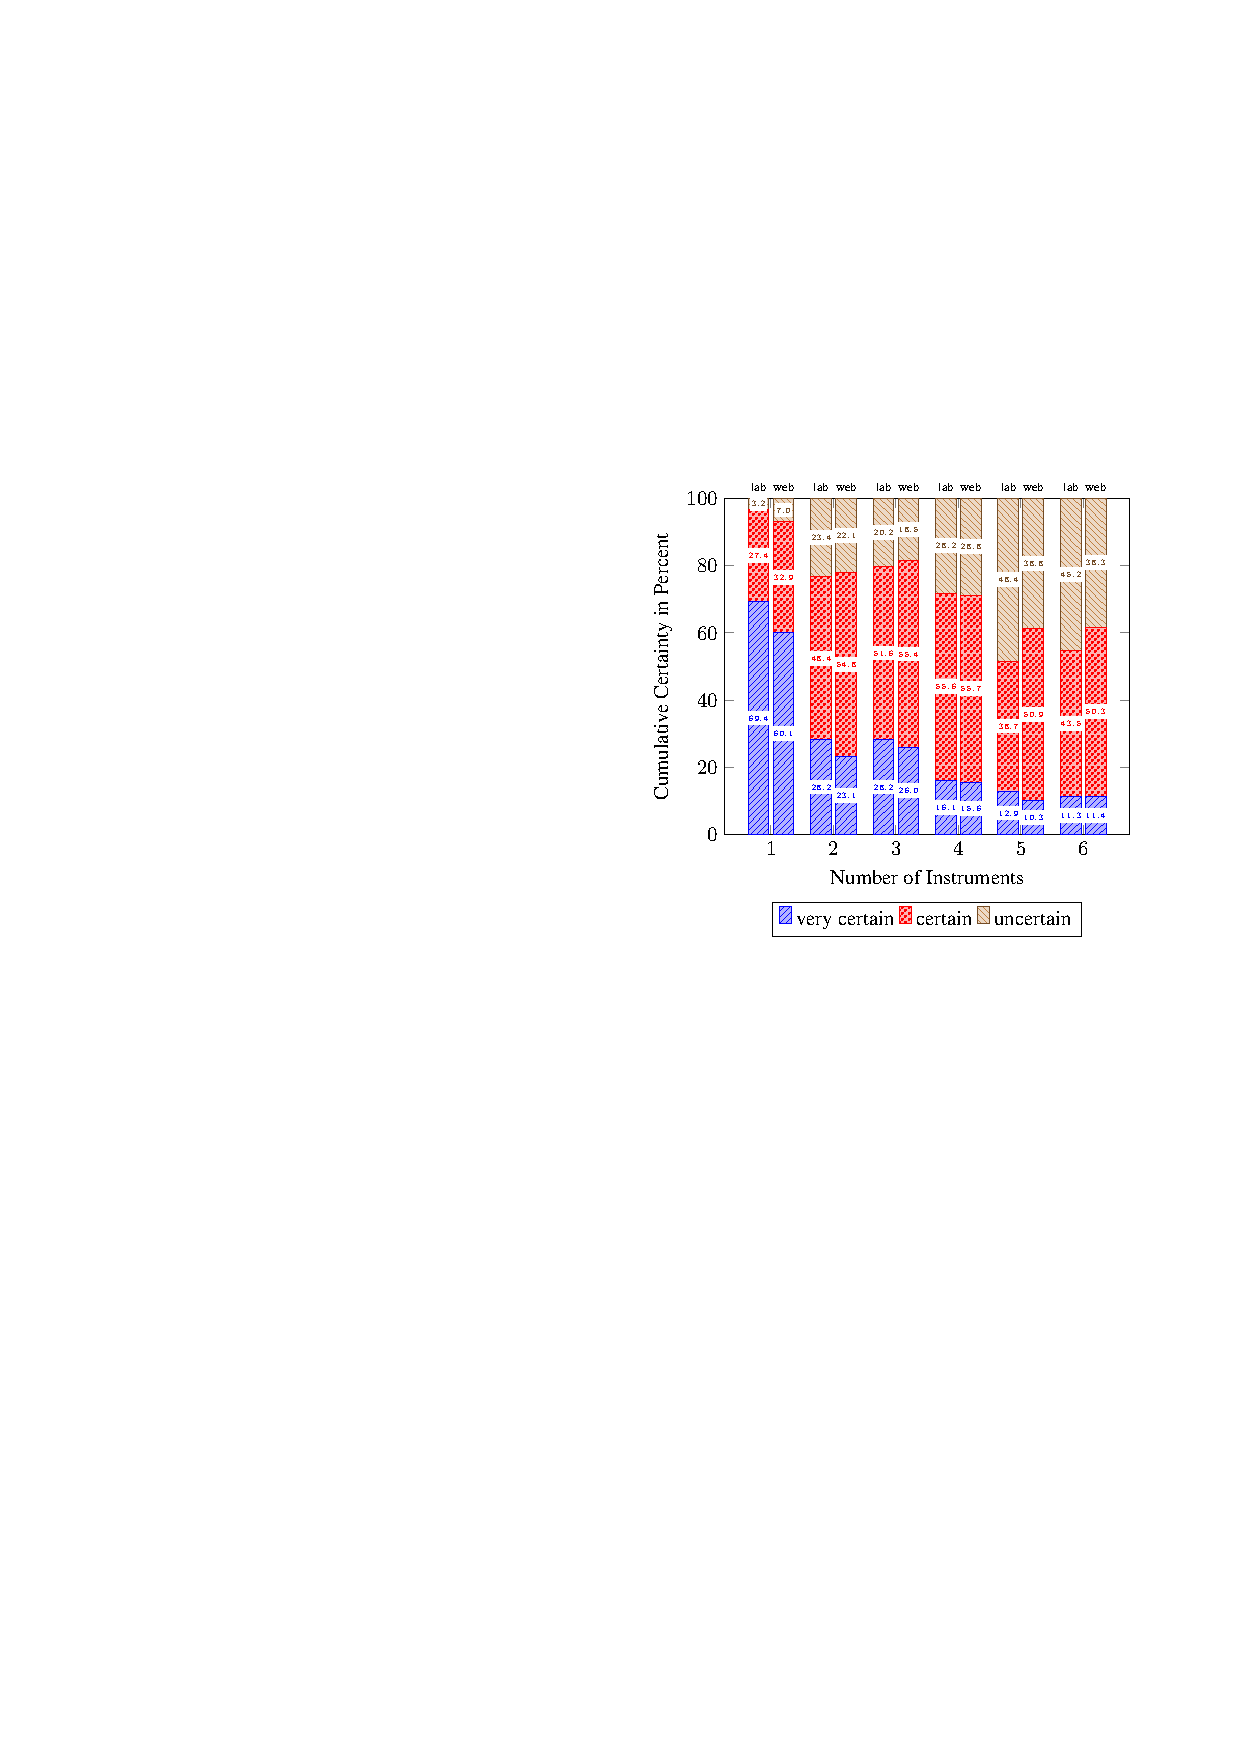
\includegraphics[width=0.45\textwidth]{Chapters/07_Analysis_Experiment/plotdata/certainty.pdf}
% \caption{Differences in certainty between the Internet experiment (web) and laboratory experiment (lab).}
% \label{figure:certainty_web_iis}
% \end{figure}

% To confirm the marginal differences between the Internet experiment and laboratory experiment for $\textit{Dev}_{\mathrm{Abs}}$, a linear regression model was calculated.
% The result tables can be found in~\cite{schoeffler13}.
% \begin{table}[h]
% \center
% \scriptsize
% \begin{tabular*}{0.45\textwidth}{p{1.5cm}ccccp{0.8cm}}
% \toprule[1.5pt]
% Coefficient & Estimate & Std. Error & z-value & p-value\\
% \midrule
% (Intercept) & 0.08535 & 0.02706 & 3.154 & 0.00161\\
% $\textit{Num}_{\mathrm{Inst}} = 2$ & 0.17683 & 0.01881 & 9.401  & \textless~2e-16\\
% $\textit{Num}_{\mathrm{Inst}} = 3$ & 0.30122 & 0.01881 & 16.014  & \textless~2e-16\\
% $\textit{Num}_{\mathrm{Inst}} = 4$ & 1.02154 & 0.01881 & 54.309  & \textless~2e-16\\
% $\textit{Num}_{\mathrm{Inst}} = 5$ & 1.67967 & 0.01881 & 89.297  & \textless~2e-16\\
% $\textit{Num}_{\mathrm{Inst}} = 6$ & 2.56667 & 0.01881 & 136.453  & \textless~2e-16\\
% $\textit{Environment} = \textrm{`}web\textrm{'}$ & 0.05481 & 0.02482 & 2.208  & 0.02724\\
% \midrule
% \multicolumn{5}{l}{Residual standard error: 0.6597 on 14753 degrees of freedom}\\
% \multicolumn{5}{l}{Multiple R-squared: 0.6603,	Adjusted R-squared: 0.6602}\\
% \multicolumn{5}{l}{F-statistic:  4779 on 6 and 14753 DF,  p-value: \textless~2.2e-16}\\
% \bottomrule[1.5pt]
% \end{tabular*}
% \caption{Linear regression model for $\textit{Dev}_{\mathrm{Abs}}$ calculated from the data obtained by the Internet experiment and the laboratory experiment.}
% \label{table:lm_absolute_deviation}
% \end{table}

% Another response variable that was obtained from the participants was the certainty of their estimation. Figure~\ref{figure:certainty_web_iis} depicts the certainty values for the Internet experiment and the laboratory experiment.

% For testing whether the environment has a significant influence on the certainty of the participants ($\textit{Certainty}$), a cumulative link model (also called ordered regression model) was calculated\cite{Christensen2012}. The cumulative link model is used since $\textit{Certainty}$ is an ordered dependent variable with the possible values `uncertain', `certain' and `very certain'. The predictor variables for the ordered regression model are $\textit{Num}_{\mathrm{Inst}}$ and $\textit{Environment}$. Again, the details of the cumulative link model for $\textit{Certainty}$ can be found in~\cite{schoeffler13}.

% \begin{table}[t]
% \center
% \scriptsize
% \begin{tabular*}{0.45\textwidth}{cccccc}
% \toprule[1.5pt]
% Coefficient & Estimate & Std. Error & z-value & p-value\\
% \midrule
% $\textit{Num}_{\mathrm{Inst}} = 2$ & -1.61273 & 0.05744 & -28.078  & \textless~2e-16\\
% $\textit{Num}_{\mathrm{Inst}} = 3$ & -1.43164 & 0.05701 & -25.114  & \textless~2e-16\\
% $\textit{Num}_{\mathrm{Inst}} = 4$ & -2.02315 & 0.05804 & -34.858  & \textless~2e-16\\
% $\textit{Num}_{\mathrm{Inst}} = 5$ & -2.47933 & 0.05901 & -42.013  & \textless~2e-16\\
% $\textit{Num}_{\mathrm{Inst}} = 6$ & -2.43573 & 0.05900 & -41.283  & \textless~2e-16\\
% $\textit{Environment} = \textrm{`}web\textrm{'}$ & -0.01008 & 0.07355 & -0.137  & 0.891\\
% \midrule
% \multicolumn{5}{l}{Threshold coefficients:}\\
% & Estimate & Std. Error & z-value &\\
% $uncertain|certain$ & -2.90465 & 0.08434 & -34.441  &\\
% $certain|very certain$ & -0.41072 & 0.08090 & -5.077  &\\
% \multicolumn{5}{l}{AIC: 28242.52}\\
% \bottomrule[1.5pt]
% \end{tabular*}
% \caption{Logit cumulative link model of certainty that was calculated from the data obtained by the Internet experiment and the laboratory experiment.}
% \label{table:olr_both}
% \end{table}
% Same as $\textit{Resp}_{\mathrm{Correct}}$, the environment of the experiment has no significant influence on the dependent variable $\textit{Certainty}$. Considering the number of participants and the comparable low coefficient, the environment had a very low influence on $\textit{Certainty}$.

% \vspace{-0.1in}
% \subsection{Discussion}\label{sec:discussion}
% \par
% In our previous result analysis of the laboratory experiment\cite{Stoter2013} we set the focus on the differences between musicians and non-musicians. Between the Internet experiment and the laboratory experiment, slightly different results were obtained when looking into how musicians and non-musicians performed (Figure~\ref{figure:error_probability_iis_vs_web}). In the laboratory experiment musicians performed much better compared to non-musicians than in the Internet Experiment. One reason seems to be that in the laboratory experiment 74.2\% of the musicians had also a professional background in audio. In the Internet experiment only 27.5\% of the musicians had a professional background in audio. Since audio professionals more often have to detect hardly audible differences in audio files they are more trained in this field. As mentioned before, being a musician in our context does just mean that the participant plays an instrument without any information about his expert level or the time he or she spends on practicing.
% \par
% When examining the responses for items with the same number of instruments being played back, noticeable differences between the genres were found. For the stimuli with $\textit{Num}_{\mathrm{Inst}} \le 4$ the mean of $\textit{Resp}_{\mathrm{Correct}}$ was $53.0\%$ and for non-classical items $62.5\%$. Since the experiment was not designed for testing classical versus non-classical items, we cannot make definitive statements about whether humans are better in estimating instruments for a specific music genre. Moreover, we did not address this issue in our result analysis.
% \par
% \par
% It is often recommended to use headphones instead of loudspeakers for Internet experiments. From the relative low average marginal effect of $\textit{Setup}$ (Table~\ref{table:data_web_lm}), it can be derived that the type of the setup had only minor effects on the results of the Internet experiment.

% In our previous result analysis of the laboratory experiment, we set the focus on the differences between musicians and non-musicians. Between the Internet experiment and the laboratory experiment, slightly different results were obtained when looking into how musicians and non-musicians performed (Figure~\ref{figure:error_probability_iis_vs_web}). In the laboratory experiment musicians performed much better compared to non-musicians than in the Internet Experiment. One reason seems to be that in the laboratory experiment 74.2\% of the musicians had also a professional background in audio. In the Internet experiment only 27.5\% of the musicians had a professional background in audio. Since audio professionals more often have to detect hardly audible differences in audio files they are more trained in this field. As mentioned before, being a musician in our context does just mean that the participant plays an instrument without any information about his expert level or the time he or she spends on practicing.
\par
One of the stimuli in the experiments consisted of a unison mixture. The results showed that $76\%$ of the participants correctly identified two instruments. Only $18\%$ of the participants underestimated by one instrument, $6\%$ overestimated by one instrument.
\par
Surprising was the small number of participants who had to be screened. We excluded 27 participants since they gave at least one non-serious response which is about 2.3\% (1195 participants remained after excluding all trials which were not the first ones). Most of these excluded participants responded with either very high numbers (e.~g. 99) or responded with zeros for their estimated number of instruments being played. We assume that especially participants who responded with zero only wanted to get an impression of the experiment.

\section{Speaker Count Estimation}%
\label{sec:count_experiment}

\marginpar{This chapter is based on the work that has been published in 2018~\cite{stoeter19} together with Soumitro Chakrabarty and Emanuël Habets.}

\begin{figure}[htb]
	\centering
		\fbox{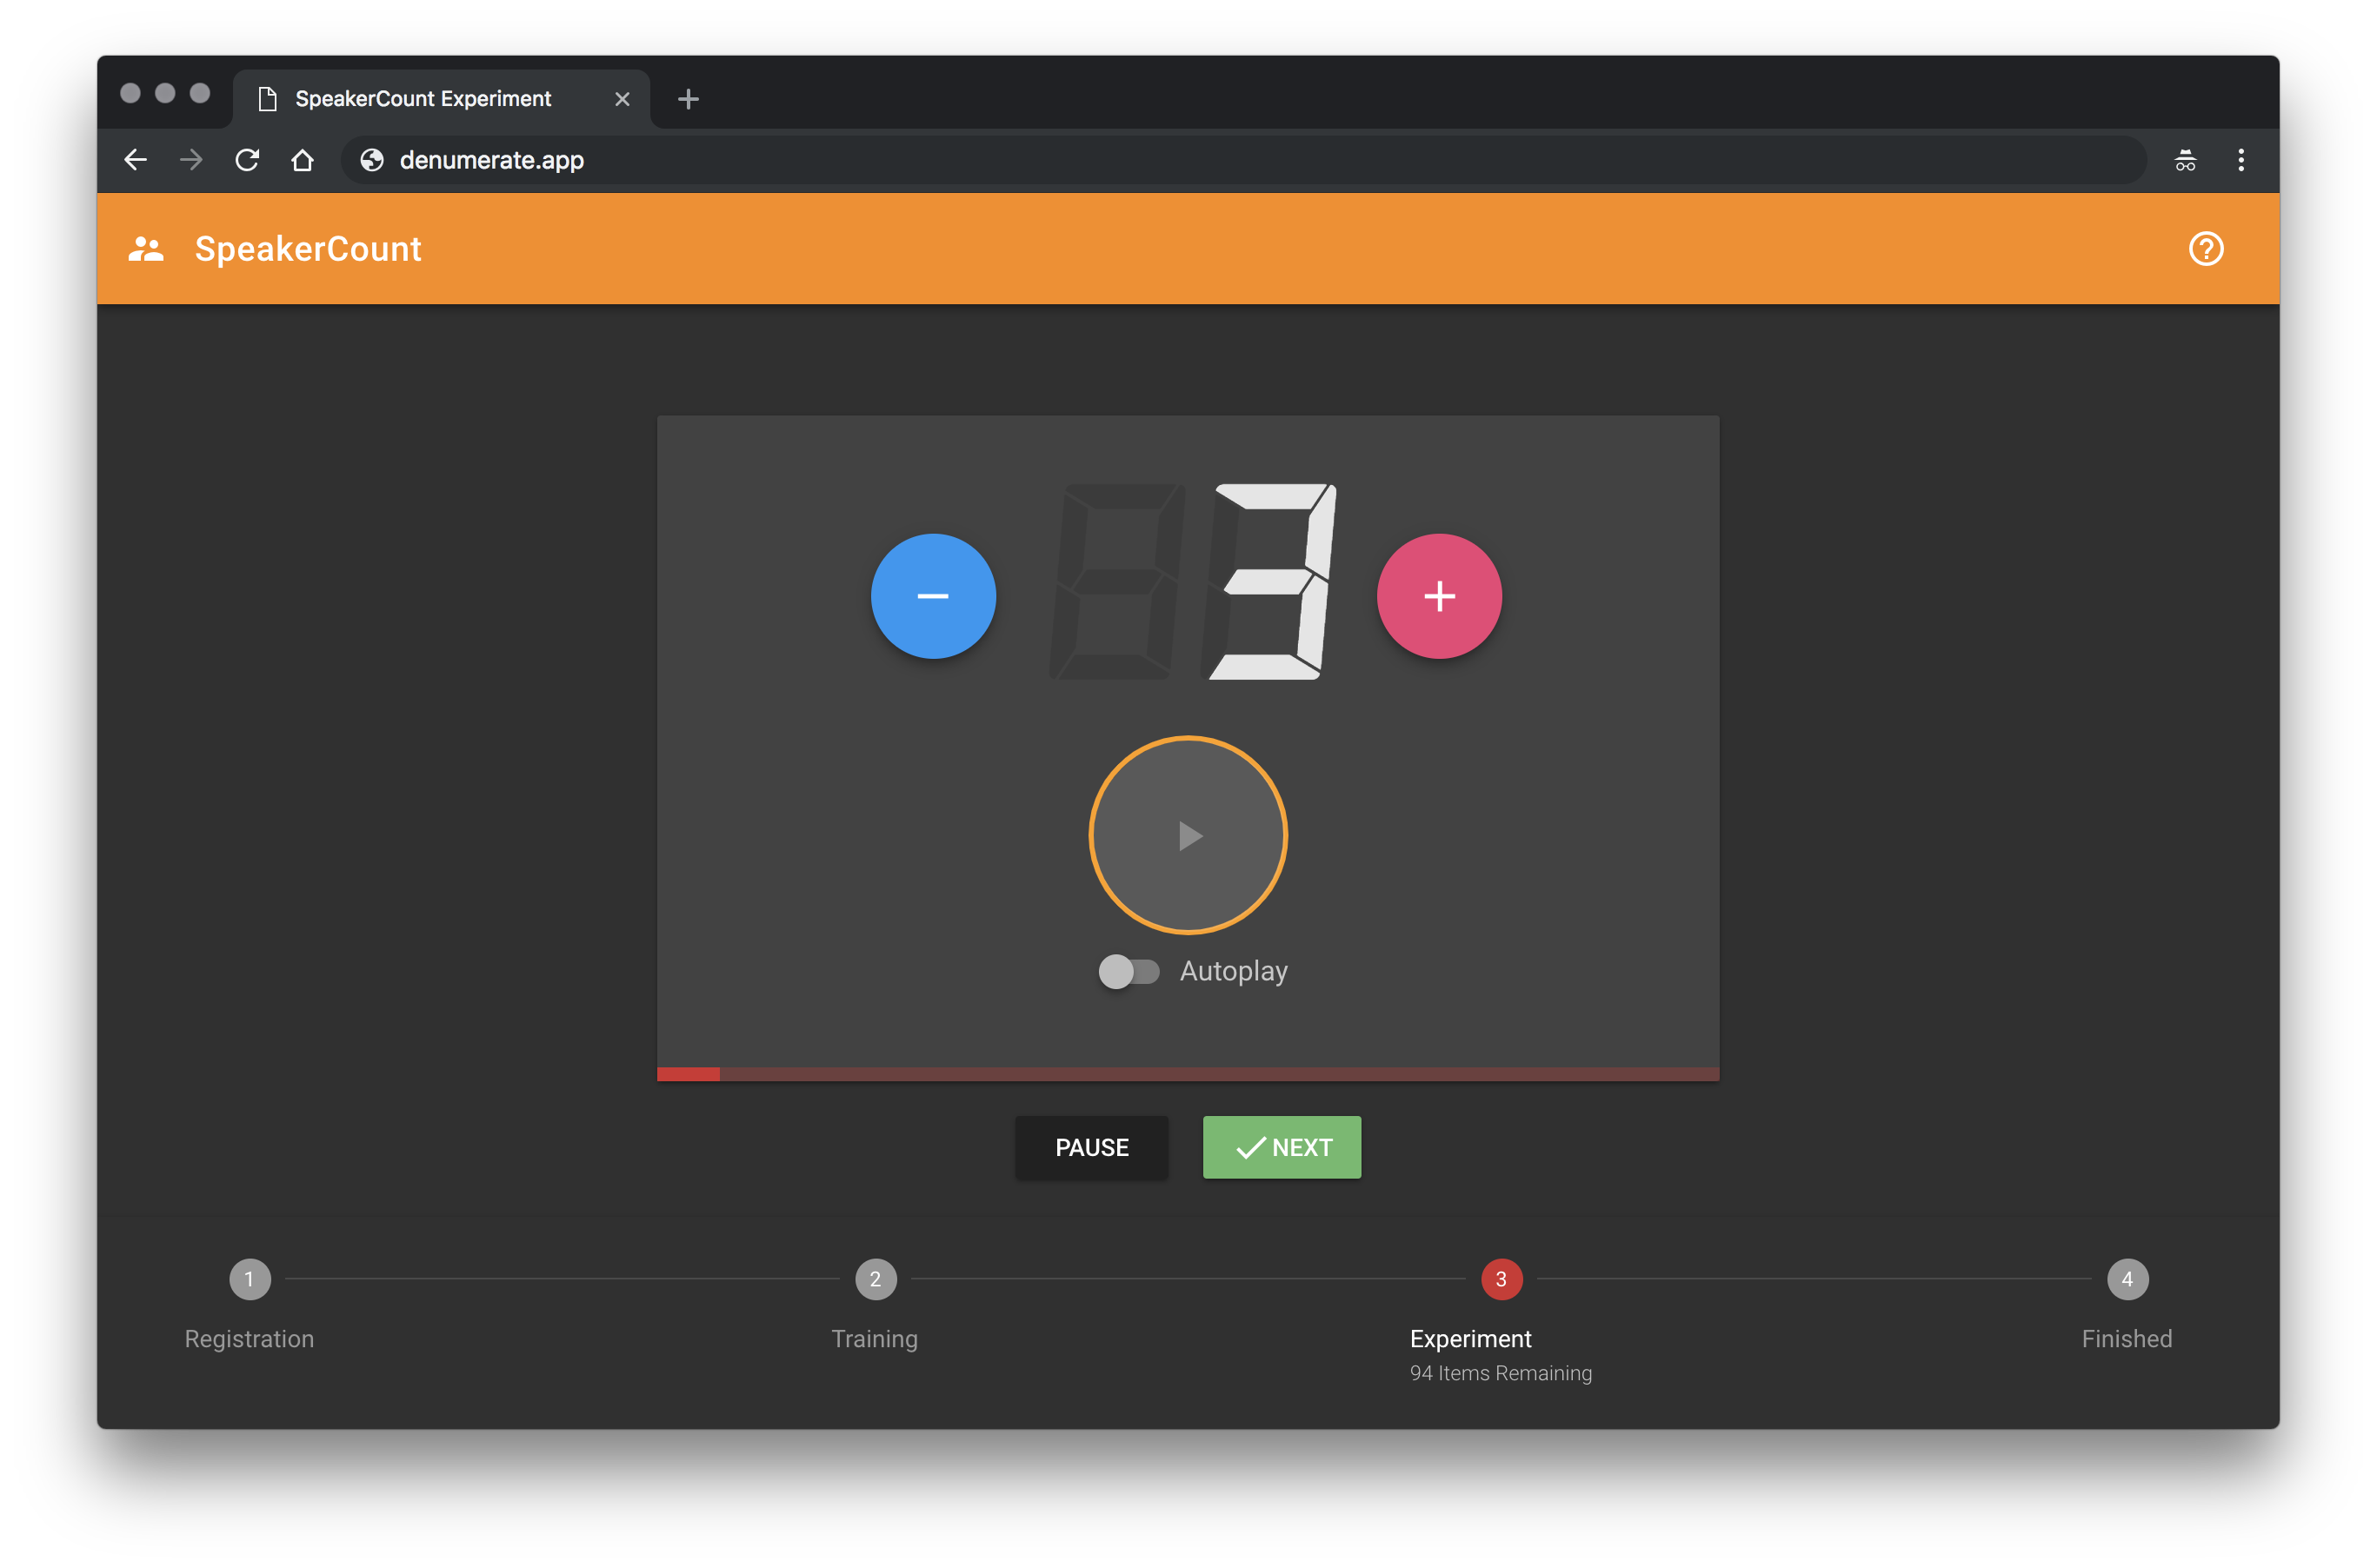
\includegraphics[width=0.8\textwidth]{Chapters/07_Analysis_Experiment/figures/experiment_ui.png}}
	\caption{Speaker count estimation experiment user interface.}
	\label{fig:user_interface_speaker}
\end{figure}

Humans are excellent in segregating one source from a mixture~\cite{bregman} and tend to use this skill to perceptually segregate speakers before they can estimate a count, as highlighted, e.g.\ in~\cite{kawashima15}.
As shown in~\cite{kashino96, kawashima15} with extensive experiments using Japanese speech samples, humans are able to correctly estimate up to three simultaneously active speakers without using any spatial cues.
In this experiment we reproduced the experiments conducted in~\cite{kawashima15, kashino96} using stimuli of English speakers.
Designed to address source separation research, we also modified the question to ask participants for ``the maximum number of concurrent speakers'' in a short excerpt of speech.

\subsection{Stimuli}
To date, many available speech datasets contain recordings where only a single speaker is active.
Datasets that include overlapped speech segments either lack accurate annotations because the annotation of speech onsets and offsets in mixtures is cumbersome for humans or lack a controlled auditory environment such as in TV/broadcasting scenarios~\cite{Gravier12}.
Since a realistic dataset of fully overlapped speakers is not available, we chose to generate synthetic mixtures.
We recognize that in a simulated ``cocktail-party'' environment, mixtures lack the conversational aspect of human communication but provide a controlled environment which helps to understand how a DNN solves the count estimation problem.
As we aim for a speaker independent solution, we selected a speech corpus with preference to a high number of different speakers instead of the number of utterances, thus increasing the number of unique mixtures.
We selected \emph{LibriSpeech clean-360}~\cite{panayotov15} which includes 363 hours of clean speech of English utterances from 921 speakers (439 female and 482 male speakers) sampled at 16 kHz.
\par
To compute the maximum number concurrent speakers \(\cardinality\), annotation of the activity of each individual speaker is required.
Even though many corpora come with word and phonemes annotation, they often are not consistent across different corpora.
We therefore generated annotations based on a voice activity detection algorithm (VAD). As we rely on a robust VAD estimate, we found the implementation from the \emph{Chromium Web Browser} as part of the WebRTC Standard\footnote{WebRTC 1.0: Real-time Communication Between Browsers W3C Editor's Draft 05 June 2017} to yield good results.
\par
To generate a single example, a tuple of a speech mixture and its ground truth speaker count \(\cardinality \), we draw a unique set of \(\cardinality \) speakers from the corpus.
For each of the speakers we then select a random utterance, resampled to 16 kHz sampling rate and apply VAD.\@
The VAD method was configured using default parameters using a hop size of 10~ms.
Further, the VAD estimate was used to remove silence from the beginning and the end of an utterance recording.
In the next step, more utterances from the same speaker are drawn from the corpus until the desired duration is reached.
We removed silence in the beginning and end of each utterance to increase the overlap within one segment.
Both, the audio recording and the VAD annotation of each utterance is concatenated.
The procedure is repeated for all speakers such that \(\cardinality \) time domain signals are created.
Signals are linearly mixed and peak normalized to avoid clipping.
The ground truth output \(\cardinality \) for each sample is then computed from the VAD matrix using the maximum of the sum over all speakers.
\par
In fact, our method to generate synthetic samples results in an average overlap for \(k=2\) of 85\% and for \(k=10\) of 55\% (based on 5s segments).
This procedure is similar to~\cite{mesaros17} used to label the data.
The Dataset is available for download~\cite{oss_libricount}.

\subsection{Experimental Setup}

We conducted the study using the simulated data from the \emph{LIBRI Count Dataset} as mentioned in the previous subsection.
In turn, we randomly selected 10 samples for each \(k \in {0, \ldots, 10}\), resulting in 100 mixtures of 5~seconds duration each.
The stimuli were presented in random order using a custom web-based interface (depicted in Figure~\ref{fig:user_interface_speaker}) connected to a database API that saved the anonymized count responses and additional information about the participant session such as the response time.
The experiment was done using \emph{between-group design}, where one group (blind experiment) did not get any prior information about the maximum number of speakers in the test set (similar to~\cite{kawashima15}).
However, the maximum number of speakers was revealed to the other group (informed experiment).
Further, none of the participants received any feedback about the error made during the trials.
The participants were able to pause and resume the experiment at any time to reduce fatigue.
Similarly to~\cite{kawashima15}, lab-based experiments were conducted with ten participants for each group (\(n=20\)) using a custom designed web-based software.
None of the participants were native English speakers.
The experiment and its results from all participants is made available through~\cite{oss_countit}.
A simplified version of the experiment is made available through a web application\footnote{\url{https://denumerate.app}} with the purpose to continuously gather data.

\subsection{Experiment Results}
To reveal over and underestimation errors, we decided to report the average response for each group of \(k\).
As a reference, we also included the average results from~\cite[Experiment 1, 5~seconds duration]{kawashima15} which shows similar (with slightly higher error probability) results compared to our blind experiment.
Also in~\cite{kawashima15} the maximum number of speakers to test was six whereas we evaluated stimuli with up to ten speakers.
The results of our lab-based experiments are shown in Figure~\ref{fig:experimentA} and Figure~\ref{fig:experimentB}.
Results indicate that underestimation becomes apparent for \(k > 3\).
First and foremost, we can confirm the ``one-two-three-many'' paradigm on our experiment with English utterances.
When we asked participants about the strategy they pursued, many reported that with more than three speakers it is not possible to identify (and count) the speakers but rather compare the \emph{density} of the speech to that of 1-3 speakers.
For higher speaker counts, participants reported that the phoneme density was a relevant cue that allowed them to extrapolate a source count estimate.
Interestingly, our results of the informed experiment reveal that they performed significantly better than those that participated blindly.
This is especially obvious for six and more speakers where the informed group performed better by more than one speaker in mean absolute deviation.

\begin{figure}[t!]
    \centering
    \begin{adjustbox}{width=0.7\columnwidth}
      % This file was created by matplotlib2tikz v0.6.13.
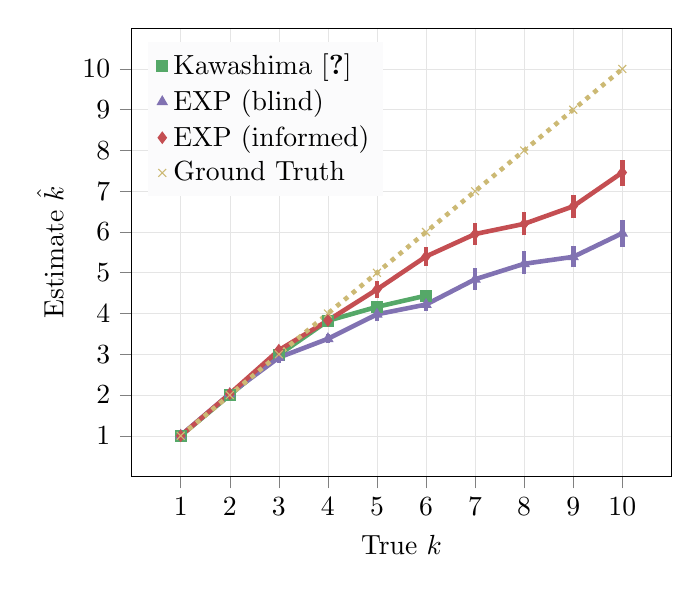
\begin{tikzpicture}

\definecolor{color1}{rgb}{0.298039215686275,0.447058823529412,0.690196078431373}
\definecolor{color0}{rgb}{0.917647058823529,0.917647058823529,0.949019607843137}
\definecolor{color4}{rgb}{0.768627450980392,0.305882352941176,0.32156862745098}
\definecolor{color2}{rgb}{0.333333333333333,0.658823529411765,0.407843137254902}
\definecolor{color5}{rgb}{0.8,0.725490196078431,0.454901960784314}
\definecolor{color3}{rgb}{0.505882352941176,0.447058823529412,0.698039215686274}

\begin{axis}[
xlabel={True \(k\)},
ylabel={Estimate \(\hat{k}\)},
xmin=-1, xmax=10,
ymin=0, ymax=11,
ytick={1,2,3,4,5,6,7,8,9,10},
xtick={0,1,2,3,4,5,6,7,8,9},
xticklabels={1,2,3,4,5,6,7,8,9,10},
tick align=outside,
tick pos=left,
ymajorgrids,
xmajorgrids,
grid style={line width=.1pt, draw=gray!20},
major grid style={line width=.2pt,draw=gray!20},
axis line style={black},
legend style={at={(0.03,0.97)}, anchor=north west, draw=none, fill=color0!20},
legend cell align={left},
legend entries={{Kawashima~\cite{kawashima15}}, {EXP (blind)}, {EXP (informed)},{Ground Truth}}
]
\addplot [only marks, mark size=2.0, mark=square*, draw=color2, fill=color2, colormap/blackwhite]
table{%
x                      y
+0.000000000000000e+00 +1.000000000000000e+00
+1.000000000000000e+00 +2.000000000000000e+00
+2.000000000000000e+00 +2.987442378071903e+00
+3.000000000000000e+00 +3.821715111593599e+00
+4.000000000000000e+00 +4.163430371330779e+00
+5.000000000000000e+00 +4.438511376242037e+00
};
\addplot [line width=1.66pt, color2, forget plot]
table {%
0 1
1 2
2 2.9874423780719
3 3.8217151115936
4 4.16343037133078
5 4.43851137624204
6 nan
7 nan
8 nan
9 nan
};
\addplot [line width=1.66pt, color2, forget plot]
table {%
0 nan
0 nan
};
\addplot [line width=1.66pt, color2, forget plot]
table {%
1 nan
1 nan
};
\addplot [line width=1.66pt, color2, forget plot]
table {%
2 nan
2 nan
};
\addplot [line width=1.66pt, color2, forget plot]
table {%
3 nan
3 nan
};
\addplot [line width=1.66pt, color2, forget plot]
table {%
4 nan
4 nan
};
\addplot [line width=1.66pt, color2, forget plot]
table {%
5 nan
5 nan
};
\addplot [line width=1.66pt, color2, forget plot]
table {%
6 nan
6 nan
};
\addplot [line width=1.66pt, color2, forget plot]
table {%
7 nan
7 nan
};
\addplot [line width=1.66pt, color2, forget plot]
table {%
8 nan
8 nan
};
\addplot [line width=1.66pt, color2, forget plot]
table {%
9 nan
9 nan
};

\addplot [only marks, mark size=2.0, mark=triangle*, draw=color3, fill=color3, colormap/blackwhite]
table{%
x                      y
+0.000000000000000e+00 +1.010000000000000e+00
+1.000000000000000e+00 +2.030000000000000e+00
+2.000000000000000e+00 +2.920000000000000e+00
+3.000000000000000e+00 +3.380000000000000e+00
+4.000000000000000e+00 +3.980000000000000e+00
+5.000000000000000e+00 +4.220000000000000e+00
+6.000000000000000e+00 +4.840000000000000e+00
+7.000000000000000e+00 +5.220000000000000e+00
+8.000000000000000e+00 +5.390000000000000e+00
+9.000000000000000e+00 +5.970000000000000e+00
};
\addplot [line width=1.66pt, color3, forget plot]
table {%
0 1.01
1 2.03
2 2.92
3 3.38
4 3.98
5 4.22
6 4.84
7 5.22
8 5.39
9 5.97
};
\addplot [line width=1.66pt, color3, forget plot]
table {%
0 1
0 1.03
};
\addplot [line width=1.66pt, color3, forget plot]
table {%
1 2
1 2.07
};
\addplot [line width=1.66pt, color3, forget plot]
table {%
2 2.78975
2 3.05
};
\addplot [line width=1.66pt, color3, forget plot]
table {%
3 3.27
3 3.5
};
\addplot [line width=1.66pt, color3, forget plot]
table {%
4 3.80975
4 4.16025
};
\addplot [line width=1.66pt, color3, forget plot]
table {%
5 4.06
5 4.4
};
\addplot [line width=1.66pt, color3, forget plot]
table {%
6 4.58
6 5.11
};
\addplot [line width=1.66pt, color3, forget plot]
table {%
7 4.97
7 5.53
};
\addplot [line width=1.66pt, color3, forget plot]
table {%
8 5.13
8 5.66
};
\addplot [line width=1.66pt, color3, forget plot]
table {%
9 5.64
9 6.29
};
\addplot [only marks, mark size=2.0, mark=diamond*, draw=color4, fill=color4, colormap/blackwhite]
table{%
x                      y
+0.000000000000000e+00 +1.000000000000000e+00
+1.000000000000000e+00 +2.030000000000000e+00
+2.000000000000000e+00 +3.100000000000000e+00
+3.000000000000000e+00 +3.830000000000000e+00
+4.000000000000000e+00 +4.590000000000000e+00
+5.000000000000000e+00 +5.400000000000000e+00
+6.000000000000000e+00 +5.950000000000000e+00
+7.000000000000000e+00 +6.200000000000000e+00
+8.000000000000000e+00 +6.630000000000000e+00
+9.000000000000000e+00 +7.460000000000000e+00
};
\addplot [line width=1.66pt, color4, forget plot]
table {%
0 1
1 2.03
2 3.1
3 3.83
4 4.59
5 5.4
6 5.95
7 6.2
8 6.63
9 7.46
};
\addplot [line width=1.66pt, color4, forget plot]
table {%
0 1
0 1
};
\addplot [line width=1.66pt, color4, forget plot]
table {%
1 1.97
1 2.1
};
\addplot [line width=1.66pt, color4, forget plot]
table {%
2 3
2 3.21
};
\addplot [line width=1.66pt, color4, forget plot]
table {%
3 3.67
3 3.98
};
\addplot [line width=1.66pt, color4, forget plot]
table {%
4 4.39
4 4.8
};
\addplot [line width=1.66pt, color4, forget plot]
table {%
5 5.16
5 5.64
};
\addplot [line width=1.66pt, color4, forget plot]
table {%
6 5.69
6 6.23
};
\addplot [line width=1.66pt, color4, forget plot]
table {%
7 5.91975
7 6.48
};
\addplot [line width=1.66pt, color4, forget plot]
table {%
8 6.34
8 6.92
};
\addplot [line width=1.66pt, color4, forget plot]
table {%
9 7.14
9 7.76025
};
\addplot [only marks, mark size=2.0, draw=color5, mark=x, fill=color5, colormap/blackwhite]
table{%
x                      y
+0.000000000000000e+00 +1.000000000000000e+00
+1.000000000000000e+00 +2.000000000000000e+00
+2.000000000000000e+00 +3.000000000000000e+00
+3.000000000000000e+00 +4.000000000000000e+00
+4.000000000000000e+00 +5.000000000000000e+00
+5.000000000000000e+00 +6.000000000000000e+00
+6.000000000000000e+00 +7.000000000000000e+00
+7.000000000000000e+00 +8.000000000000000e+00
+8.000000000000000e+00 +9.000000000000000e+00
+9.000000000000000e+00 +1.000000000000000e+01
};
\addplot [line width=1.66pt, color5, dotted, forget plot]
table {%
0 1
1 2
2 3
3 4
4 5
5 6
6 7
7 8
8 9
9 10
};
\addplot [line width=1.66pt, color5, forget plot]
table {%
0 nan
0 nan
};
\addplot [line width=1.66pt, color5, forget plot]
table {%
1 nan
1 nan
};
\addplot [line width=1.66pt, color5, forget plot]
table {%
2 nan
2 nan
};
\addplot [line width=1.66pt, color5, forget plot]
table {%
3 nan
3 nan
};
\addplot [line width=1.66pt, color5, forget plot]
table {%
4 nan
4 nan
};
\addplot [line width=1.66pt, color5, forget plot]
table {%
5 nan
5 nan
};
\addplot [line width=1.66pt, color5, forget plot]
table {%
6 nan
6 nan
};
\addplot [line width=1.66pt, color5, forget plot]
table {%
7 nan
7 nan
};
\addplot [line width=1.66pt, color5, forget plot]
table {%
8 nan
8 nan
};
\addplot [line width=1.66pt, color5, forget plot]
table {%
9 nan
9 nan
};
\end{axis}

\end{tikzpicture}

    \end{adjustbox}
    \caption{Average responses in comparison to the results of \emph{Kawashima}~\cite{kawashima15}. Error bars show 95\% confidence intervals (not available for~\cite{kawashima15}).}%
    \label{fig:experimentA}
 \end{figure}

\begin{figure}[t!]
   \centering
   \begin{adjustbox}{width=0.7\columnwidth}
     % This file was created by matplotlib2tikz v0.6.14.
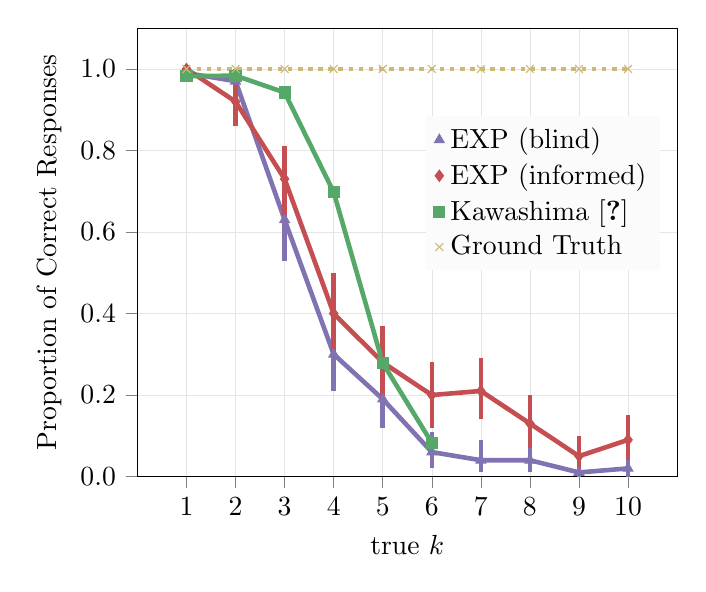
\begin{tikzpicture}

\definecolor{color1}{rgb}{0.298039215686275,0.447058823529412,0.690196078431373}
\definecolor{color0}{rgb}{0.917647058823529,0.917647058823529,0.949019607843137}
\definecolor{color4}{rgb}{0.768627450980392,0.305882352941176,0.32156862745098}
\definecolor{color2}{rgb}{0.333333333333333,0.658823529411765,0.407843137254902}
\definecolor{color5}{rgb}{0.8,0.725490196078431,0.454901960784314}
\definecolor{color3}{rgb}{0.505882352941176,0.447058823529412,0.698039215686274}

\begin{axis}[
xlabel={true $k$},
ylabel={Proportion of Correct Responses},
xmin=-1, xmax=10,
ymin=0, ymax=1.1,
ymajorgrids,
xmajorgrids,
xtick={0,1,2,3,4,5,6,7,8,9},
xticklabels={1,2,3,4,5,6,7,8,9,10},
ytick={0,0.2,0.4,0.6,0.8,1},
yticklabels={0.0,0.2,0.4,0.6,0.8,1.0},
tick align=outside,
tick pos=left,
grid style={line width=.1pt, draw=gray!20},
major grid style={line width=.2pt,draw=gray!20},
axis line style={black},
legend entries={{EXP (blind)},{EXP (informed)},{Kawashima~\cite{kawashima15}},{Ground Truth}},
legend cell align={left},
legend style={at={(0.97,0.46)}, anchor=south east, draw=none, fill=color0!20}
]
\addplot [only marks, mark size=2.0, mark=triangle*, draw=color3, fill=color3, colormap/blackwhite]
table{%
x                      y
+0.000000000000000e+00 +9.900000000000000e-01
+1.000000000000000e+00 +9.700000000000000e-01
+2.000000000000000e+00 +6.300000000000000e-01
+3.000000000000000e+00 +3.000000000000000e-01
+4.000000000000000e+00 +1.900000000000000e-01
+5.000000000000000e+00 +6.000000000000000e-02
+6.000000000000000e+00 +4.000000000000000e-02
+7.000000000000000e+00 +4.000000000000000e-02
+8.000000000000000e+00 +1.000000000000000e-02
+9.000000000000000e+00 +2.000000000000000e-02
};
\addplot [line width=1.66pt, color3, forget plot]
table {%
0 0.99
1 0.97
2 0.63
3 0.3
4 0.19
5 0.06
6 0.04
7 0.04
8 0.01
9 0.02
};
\addplot [line width=1.66pt, color3, forget plot]
table {%
0 0.97
0 1
};
\addplot [line width=1.66pt, color3, forget plot]
table {%
1 0.93
1 1
};
\addplot [line width=1.66pt, color3, forget plot]
table {%
2 0.53
2 0.72
};
\addplot [line width=1.66pt, color3, forget plot]
table {%
3 0.21
3 0.39025
};
\addplot [line width=1.66pt, color3, forget plot]
table {%
4 0.12
4 0.27
};
\addplot [line width=1.66pt, color3, forget plot]
table {%
5 0.02
5 0.11
};
\addplot [line width=1.66pt, color3, forget plot]
table {%
6 0.01
6 0.09
};
\addplot [line width=1.66pt, color3, forget plot]
table {%
7 0.01
7 0.08
};
\addplot [line width=1.66pt, color3, forget plot]
table {%
8 0
8 0.03
};
\addplot [line width=1.66pt, color3, forget plot]
table {%
9 0
9 0.05
};
\addplot [only marks, mark size=2.0, mark=diamond*, draw=color4, fill=color4, colormap/blackwhite]
table{%
x                      y
+0.000000000000000e+00 +1.000000000000000e+00
+1.000000000000000e+00 +9.200000000000000e-01
+2.000000000000000e+00 +7.300000000000000e-01
+3.000000000000000e+00 +4.000000000000000e-01
+4.000000000000000e+00 +2.800000000000000e-01
+5.000000000000000e+00 +2.000000000000000e-01
+6.000000000000000e+00 +2.100000000000000e-01
+7.000000000000000e+00 +1.300000000000000e-01
+8.000000000000000e+00 +5.000000000000000e-02
+9.000000000000000e+00 +9.000000000000000e-02
};
\addplot [line width=1.66pt, color4, forget plot]
table {%
0 1
1 0.92
2 0.73
3 0.4
4 0.28
5 0.2
6 0.21
7 0.13
8 0.05
9 0.09
};
\addplot [line width=1.66pt, color4, forget plot]
table {%
0 1
0 1
};
\addplot [line width=1.66pt, color4, forget plot]
table {%
1 0.86
1 0.97
};
\addplot [line width=1.66pt, color4, forget plot]
table {%
2 0.64
2 0.81
};
\addplot [line width=1.66pt, color4, forget plot]
table {%
3 0.3
3 0.5
};
\addplot [line width=1.66pt, color4, forget plot]
table {%
4 0.19
4 0.37
};
\addplot [line width=1.66pt, color4, forget plot]
table {%
5 0.12
5 0.28
};
\addplot [line width=1.66pt, color4, forget plot]
table {%
6 0.14
6 0.29
};
\addplot [line width=1.66pt, color4, forget plot]
table {%
7 0.07
7 0.2
};
\addplot [line width=1.66pt, color4, forget plot]
table {%
8 0.01
8 0.1
};
\addplot [line width=1.66pt, color4, forget plot]
table {%
9 0.04
9 0.15
};

\addplot [only marks, mark size=2.0, mark=square*, draw=color2, fill=color2, colormap/blackwhite]
table{%
x                      y
+0.000000000000000e+00 +9.822222212577160e-01
+1.000000000000000e+00 +9.837037209040648e-01
+2.000000000000000e+00 +9.422222190875770e-01
+3.000000000000000e+00 +6.977777613811720e-01
+4.000000000000000e+00 +2.785184612911492e-01
+5.000000000000000e+00 +8.296289512602513e-02
};
\addplot [line width=1.66pt, color2, forget plot]
table {%
0 0.982222221257716
1 0.983703720904065
2 0.942222219087577
3 0.697777761381172
4 0.278518461291149
5 0.0829628951260251
6 nan
7 nan
8 nan
9 nan
};
\addplot [line width=1.66pt, color2, forget plot]
table {%
0 nan
0 nan
};
\addplot [line width=1.66pt, color2, forget plot]
table {%
1 nan
1 nan
};
\addplot [line width=1.66pt, color2, forget plot]
table {%
2 nan
2 nan
};
\addplot [line width=1.66pt, color2, forget plot]
table {%
3 nan
3 nan
};
\addplot [line width=1.66pt, color2, forget plot]
table {%
4 nan
4 nan
};
\addplot [line width=1.66pt, color2, forget plot]
table {%
5 nan
5 nan
};
\addplot [line width=1.66pt, color2, forget plot]
table {%
6 nan
6 nan
};
\addplot [line width=1.66pt, color2, forget plot]
table {%
7 nan
7 nan
};
\addplot [line width=1.66pt, color2, forget plot]
table {%
8 nan
8 nan
};
\addplot [line width=1.66pt, color2, forget plot]
table {%
9 nan
9 nan
};
\addplot [only marks, mark size=2.0, draw=color5, mark=x, fill=color5, colormap/blackwhite]
table{%
x                      y
+0.000000000000000e+00 +1.000000000000000e+00
+1.000000000000000e+00 +1.000000000000000e+00
+2.000000000000000e+00 +1.000000000000000e+00
+3.000000000000000e+00 +1.000000000000000e+00
+4.000000000000000e+00 +1.000000000000000e+00
+5.000000000000000e+00 +1.000000000000000e+00
+6.000000000000000e+00 +1.000000000000000e+00
+7.000000000000000e+00 +1.000000000000000e+00
+8.000000000000000e+00 +1.000000000000000e+00
+9.000000000000000e+00 +1.000000000000000e+00
};
\addplot [line width=1.66pt, color5, dotted, forget plot]
table {%
0 1
1 1
2 1
3 1
4 1
5 1
6 1
7 1
8 1
9 1
};
\addplot [line width=1.66pt, color5, dotted, forget plot]
table {%
0 nan
0 nan
};
\addplot [line width=1.66pt, color5, dotted, forget plot]
table {%
1 nan
1 nan
};
\addplot [line width=1.66pt, color5, dotted, forget plot]
table {%
2 nan
2 nan
};
\addplot [line width=1.66pt, color5, dotted, forget plot]
table {%
3 nan
3 nan
};
\addplot [line width=1.66pt, color5, dotted, forget plot]
table {%
4 nan
4 nan
};
\addplot [line width=1.66pt, color5, dotted, forget plot]
table {%
5 nan
5 nan
};
\addplot [line width=1.66pt, color5, dotted, forget plot]
table {%
6 nan
6 nan
};
\addplot [line width=1.66pt, color5, dotted, forget plot]
table {%
7 nan
7 nan
};
\addplot [line width=1.66pt, color5, dotted, forget plot]
table {%
8 nan
8 nan
};
\addplot [line width=1.66pt, color5, dotted, forget plot]
table {%
9 nan
9 nan
};
\end{axis}

\end{tikzpicture}

   \end{adjustbox}
   \caption{Mean probability of correct responses in comparison to the results of \emph{Kawashima}~\cite{kawashima15}. Error bars show 95\% confidence intervals (not available for~\cite{kawashima15}).}%
   \label{fig:experimentB}
\end{figure}


\section{Summary and Discussion}

% [X] A summary of findings and limitations
% [ ] Practical applications/implications
% [X] Recommendations for further research

In this chapter we presented two experiments that we conducted to get a better understanding of the human ability of estimating the number of sources in overlapped mixtures.
\par
First, we showed that estimating the number of instruments in music mixtures is a challenging task for humans.
We presented the results of a controlled experiment with 62 participants, listening to stimuli of inhomogeneous timbres.
Our experiment indicated that the upper limit is reached with more than three instruments, related to an earlier experiment~\cite{huron89} focused on voices instead of instruments.
In Chapter~\ref{cha:fundamentals}, two different questions were introduced how to frame the count estimation problem.
In this experiment, we explicitly used an open question of ``How many instruments can you hear'' to gather more knowledge into the strategies being applied by the participants.
Another reason was that the stimuli durations were too long to ask for the maximum number of concurrent stimuli, thus promoting ``counting by detection'' as a good strategy to approach the problem.\par
By comparing musicians to non-musicians, we showed that there is a significant difference in performance for count estimation, confirming similar findings in other auditory tasks~\cite{kishon01}.
Particularly, we found a that this gap is most prominent for stimuli of three and four instruments.
Furthermore, for all stimuli (ranging from one to six instruments) we revealed that musicians performed about 20\% better than non-musicians, hence revealing a ``gap of one instrument'' in mean absolute error.
\par
We then repeated this experiment in an open, uncontrolled environment with more than 1000 participants.
To our knowledge this was the first larger crowd sourced auditory experiment within the Signal Processing or MIR community.
Regarding the ability of estimating the number of instruments, the web experiment and the laboratory experiment share the same outcome: the probability to correctly estimate up to about three instruments is higher than 50\%.
These results were surprising because many participants did not use professional audio equipment.
In comparison to audio quality experiments like MUSHRA~\cite{recommendation2001MUSHRA}, we can therefore conclude that count estimation tasks are suitable for highly scalable crowd sourced listening experiments.
\par
In our second experiment we reproduced an earlier study presented in~\cite{kawashima15} to estimate the maximum number of concurrent speakers in short audio mixtures, simulating a ``cocktail-party'' environment.
Our experiment went a step further with respect to the maximum amount of speakers to be estimated (up two \(k=10\)).
The results indicated almost no person was able to correctly estimate up to ten speakers.
However, we also observed that even for more than seven speakers the mean response did further (but not linearly) increase.
This indicates that humans are possibly interpolating some sort of a speech density to make up their decision.
\par
We conclude that all of our count experiments share the same results: A) humans are unable to correctly estimate more than four sources and B), underestimation is the main cause of error.
Also we revealed that source count estimation studies can be easily be participated by non-professional listeners.